%%%%%%%%%%%%%%%%%%%%%%%%%%%%%%%%%%%%%%%%%%%%
%%%%%%%%%%%%%%%%%%%%%%%%%%%%%%%%
\chapter{Holomorphie}
La notion de dérivée d'une fonction dans le plan complexe est définie dans ce chapitre. Il sera montré plus loin qu'une application différentiable dans $\C$ possède des propriétés très particulières.

\section{Fonction d'une variable complexe}
Une fonction d'une variable complexe se définit de manière assez similaire à une fonction d'une variable réelle. Si $D$ est un domaine de $\C$, une fonction $f$ sur $D$ assigne à chaque $z \in D$ un nombre complexe $w$ appelé image de $z$ par $f$. On peut écrire $w = f(z) = u+iv$

\section{Rappels de calcul différentiel}

\subsection{Différentiabilité d'une application entre deux espaces vectoriels}

De façon générale, la différentiabilité en un point $x_0$ d'une application $f$ entre espaces vectoriels normés se traduit par l'existence d'un modèle affine continu approchant $f$ au voisinage de $x_0$.
\begin{defn}
Soient $E,F$ deux espaces vectoriels normés et soit $x_0$ un point de $E$. On dira que deux couples $(U,f),(V,g)$, avec $U,V$ voisinages ouverts de $x_0$ et $f\colon U \to F$,$g \colon V \to F$ applications continues, ont même germe en $x_0$ si et seulement si il existe un ouvert $W \subset U \cap V$ tel que $f\rvert_{W}=g\rvert_{W}$.
\end{defn}
\begin{prop}
La relation $(U,f) \sim_{x_0} (V,g)$ si et seulement si les deux couples ont même germe en $x_0$ est une relation d'équivalence. L'ensemble quotient $\{(U,f)\} / \sim_{x_0}$ est appelé ensemble des germes d'applications continues en $x_0$ à valeurs dans $F$ 
\end{prop}
\begin{defn}
Soit $E$ un espace vectoriel normé et $x_0$ un point de $E$. Soit $(U,g)$ un germe d'application continue en $x_0$ à valeurs dans $\R^+$ . On dira qu'un germe en $x_0$ $(V,f)$ à valeurs dans $F$, espace vectoriel normé,  est négligeable devant $(U,g)$ si pour tout $\epsilon > 0$, il existe un voisinage ouvert $W$ de $x_0$ inclus dans $U\cap V$ et tel que:
\[
\forall x \in W, \, \|f(x)\| < \epsilon g(x)
\]
L'ensemble des germes négligeables devant $(U,g)$ est noté $o_{x_0}(g)$.
\end{defn}
\begin{rem}
Il est important de bien prendre garde au fait que la notation $o$ désigne en réalité un ensemble de germes d'applications. On omet le plus souvent l'ouvert $U$ qui est implicite. \end{rem}
\begin{fdefn}
Soient $E,F$ deux espaces vectoriels normés sur un corps $\mathbb{K}$
 et soit $U$ un ouvert de $E$. On dira que $f \colon U \to F$ est différentiable en $x_0 \in U$ si il existe une application continue $L \colon E \to F$ et un voisinage ouvert $V$ de $x_0$ tels que:
 \[
 \forall x \in U \cap V, \, f(x) = f(x_0) + L(x-x_0) + o(\|x-x_0\|_E)
 \]
\end{fdefn}
\begin{rem}
La continuité de $L$ n'est pas une conséquence de la linéarité comme en dimension finie. 
\end{rem}
L'application $ x \mapsto f(x_0) + L(x-x_0)$ est appelée application affine tangente à $f$ en $x_0$.
\begin{prop}
Lorsqu'elle existe, l'application linéaire $L$ est unique.
\end{prop}
\begin{proof}
Supposons l'existence de deux applications linéaires  $L_1, L_2$ vérifiant la relation de définition. On pose $L =  L_1 - L_2$.Pour tout $\epsilon > 0$, il existe un ouvert $W \subset U \cap V$ tel que:
\[
\forall x \in W, \|L(x-x_0)\|_F < \epsilon \| x-x_0 \|_E
\]
Par linéarité, ceci implique:
\[
\forall v \in F, \|v\|_E = 1 \Rightarrow \|L v \|_F < \epsilon 
\]
et donc par passage à la limite:
\[
\forall v \in F, \|v\|_E = 1 \Rightarrow \|L v \|_F = 0
\]
prouvant ainsi que $L$ est l'application nulle.
\end{proof}
\subsection{Différentiabilité d'une application de $\R^2$ dans $\R^2$}
\begin{fdefn}\label{def:1.2}
Soit $U \subset \R^2$ un ouvert et soit une application $f \colon U \to \R^2$.
On dira que $f$ est différentiable en $z_0 \in U$ si il existe une application $\R$-linéaire $ L \colon \R^2 \to \R^2$ telle que :
\[f(z)=f(z_0) + L(z-z_0) + o(\|z-z_0\|_E),\]
\end{fdefn}


%On a nécessairement $A(x_0)=f(x_0)$. En effet, par définition de l'ensemble $o(\|x-x_0\|)$, il existe un voisinage $U$ de $x_0$ tel que:
%\[
%\forall x \in U, \, \|f(x)-A(x)\| \leq \|x-x_0\|
%\]
%et la propriété s'ensuit en prenant $x=x_0$.



%On fait le plus souvent l'abus de notation consistant à confondre \textbf{l'ensemble} $ o(\|x-x_0\|)$ avec un de ses éléments, pour écrire la relation entre $f$ et $H$  au voisinage de $x_0$ sous la forme:
%\[
%f(x) = f(x_0) + H(x-x_0) + o(\|x-x_0\|)
%\]
%Cette notation est la plus courante, mais se révèle parfois source d'erreurs: il faut toujours garder à l'esprit
%que le terme $o(\|x-x_0\|)$ est en fait une \textbf{fonction} négligeable devant $\|x-x_0\|$ au voisinage de $x_0$.
On notera le plus souvent $L$ par $Df(z_0)$ ou $f^\prime(z_0)$ ; il faut garder à l'esprit que ces notations désignent des applications linéaires.
%
%Lorsqu'une application est différentiable en un point, elle y est bien représentée par une application linéaire et hérite de certaines de ses propriétés, dont la continuité, comme le montre la proposition ci-dessous:
\begin{fprop}\label{prop:1.1}
Si $f \colon U \to \R^2$ est différentiable en $z_0$, alors $f$ est continue en $z_0$.
\end{fprop}
\begin{proof}
Soit $\epsilon > 0$. Il existe un $\delta >0$ tel que :
\[ \forall z \in D(z_0,\delta), \, \lvert f(z) - f(z_0) -Df(z_0)\cdot(z-z_0) \rvert \leq \epsilon \|z-z_0\|.\]
Par un argument classique,
\[\lvert f(z) -f(z_0)\rvert \leq \left(\epsilon + \|Df(z_0)\| \right)\lvert (z-z_0) \rvert,\]
où $\|Df(z_0)\|$ est la norme de l'application linéaire, c.-à-d. 
\[ \|Df(z_0)\| = \sup_{v \neq 0} \frac{\|Df(z_0) \cdot v\|}{\|v\|}.\]
\end{proof}

Lorsqu'une application est différentiable en tout point d'un ouvert $U$, on dit plus simplement qu'elle est différentiable sur $U$. Il est alors d'usage de noter l'application linéaire tangente à $f$ en $z$ par $f^\prime(z)$. On définit ainsi, une application $z \mapsto f^\prime(z)$, que nous noterons simplement $f^\prime$ : 
\[ f^\prime \colon  U \mapsto \mathcal{L}(\R^2 ; \R^2)\]
de l'ouvert $U$ dans l'ensemble $\mathcal{L}(\R^2 ; \R^2)$ des endomorphismes linéaires de $\R^2$. C'est par définition, \textit{l'application dérivée} de $f$. Il est alors possible d'étudier la continuité de $f^\prime$ en munissant l'espace vectoriel des endomorphismes de $\R^2$ de la norme d'opérateur définie ci-dessus.


\begin{fdefn}
L'application $f \colon U \to \R^2$ est dite continûment différentiable sur $U$, ou de classe $C^1$ si
\begin{enumerate}
\item $f$ est différentiable dans $U$, c.-à-d. différentiable en tout point de $U$ ;
\item l'application dérivée $f^\prime \colon U \to \mathcal{L}(\R^2 ; \R^2)$ est continue.
\end{enumerate}  
\end{fdefn}

Pour conclure cette section, mentionnons une propriété importante d'un domaine $\Omega$
\begin{fprop} Soit $f$ une application qui est $C^1$ sur un domaine $\Omega \subset \C$. Si sa dérivée $f^\prime$ est identiquement nulle dans $\Omega$, alors $f$ est constante.
\end{fprop}

Si un ouvert $U$ n'est pas connexe, par exemple la réunion de deux ouverts connexes non-vides et disjoints $U_1$ et $U_2$, alors une fonction $C^1$ constante sur chacune des composantes connexes, mais avec des valeurs différentes, aura sa dérivée nulle sur $U$. En quelque sorte, il est toujours possible de considérer de façon indépendante, le comportement d'une fonction sur chacune des composantes connexes de son ouvert de définition. 


%\subsection{Interprétation géométrique}
%
%Un endomorphisme de $\R^2$ se représente comme une transformation du plan. Étant linéaire, elle agira sur un segment de droite pour donner un autre segment de droite. La figure \ref{fig:trlin} donne un exemple de l'action d'un endomorphisme du plan sur une grille uniforme ; on notera en particulier que la déformation préserve les parties droites.
%\begin{figure}[ht]
%\centering
%\begin{subfigure}[b]{0.45\textwidth}
%
\includegraphics[width=\textwidth]{images/ima1.png}
%\caption{Grille initiale}
%\label{fig:uni_mesh}
%\end{subfigure}
%\begin{subfigure}[b]{0.45\textwidth}
%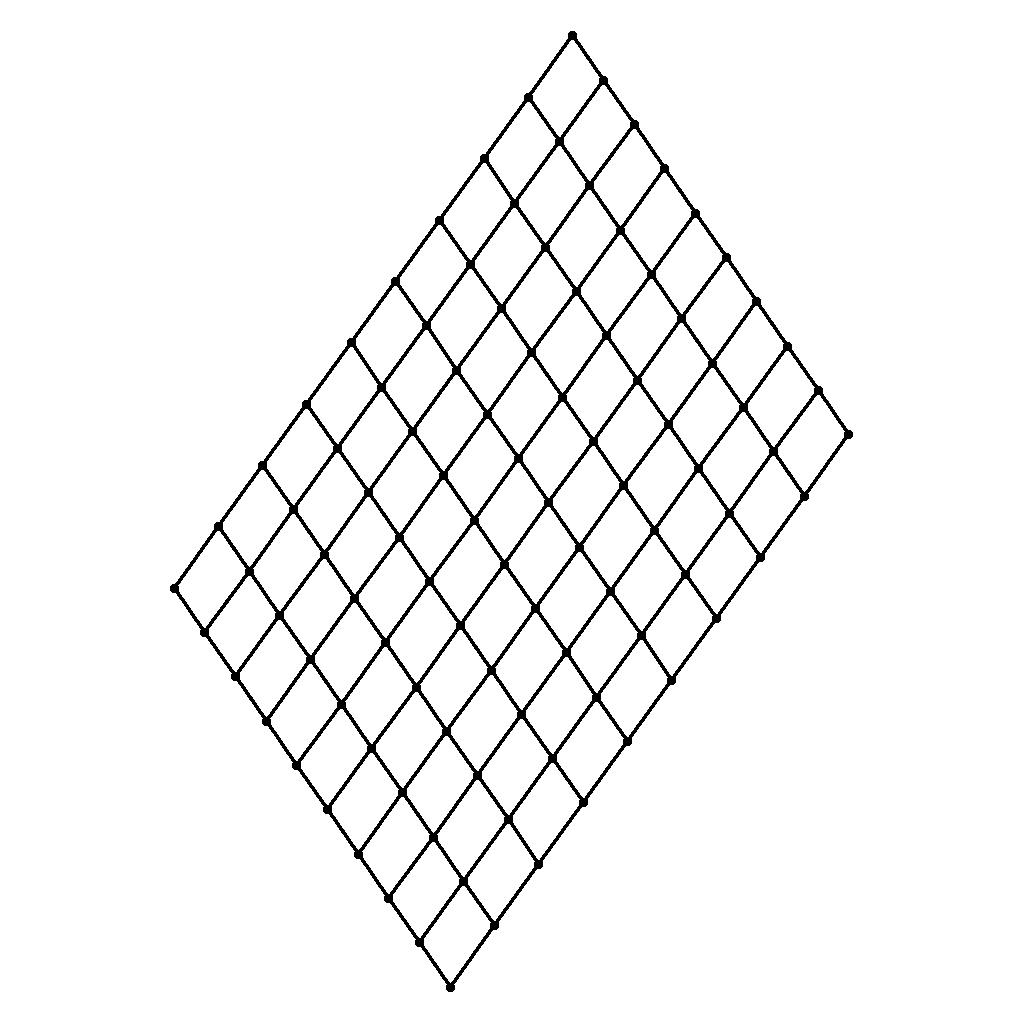
\includegraphics[width=\textwidth]{images/ima2.png}
%\caption{Grille Transformée}
%\label{fig:trlin_mesh}
%\end{subfigure}
%\caption{Transformation linéaire}\label{fig:trlin}
%\end{figure}
%A contrario, une application quelconque de $\R^2$ dans lui-même pourra donner des résultats notablement différents, tel  que celui présenté en figure \ref{fig:trnlin}
%\begin{figure}[ht]
%\centering
%\begin{subfigure}[b]{0.45\textwidth}
%
\includegraphics[width=\textwidth]{images/ima1.png}
%\caption{Grille initiale}
%\label{fig:uni_mesh}
%\end{subfigure}
%\begin{subfigure}[b]{0.45\textwidth}
%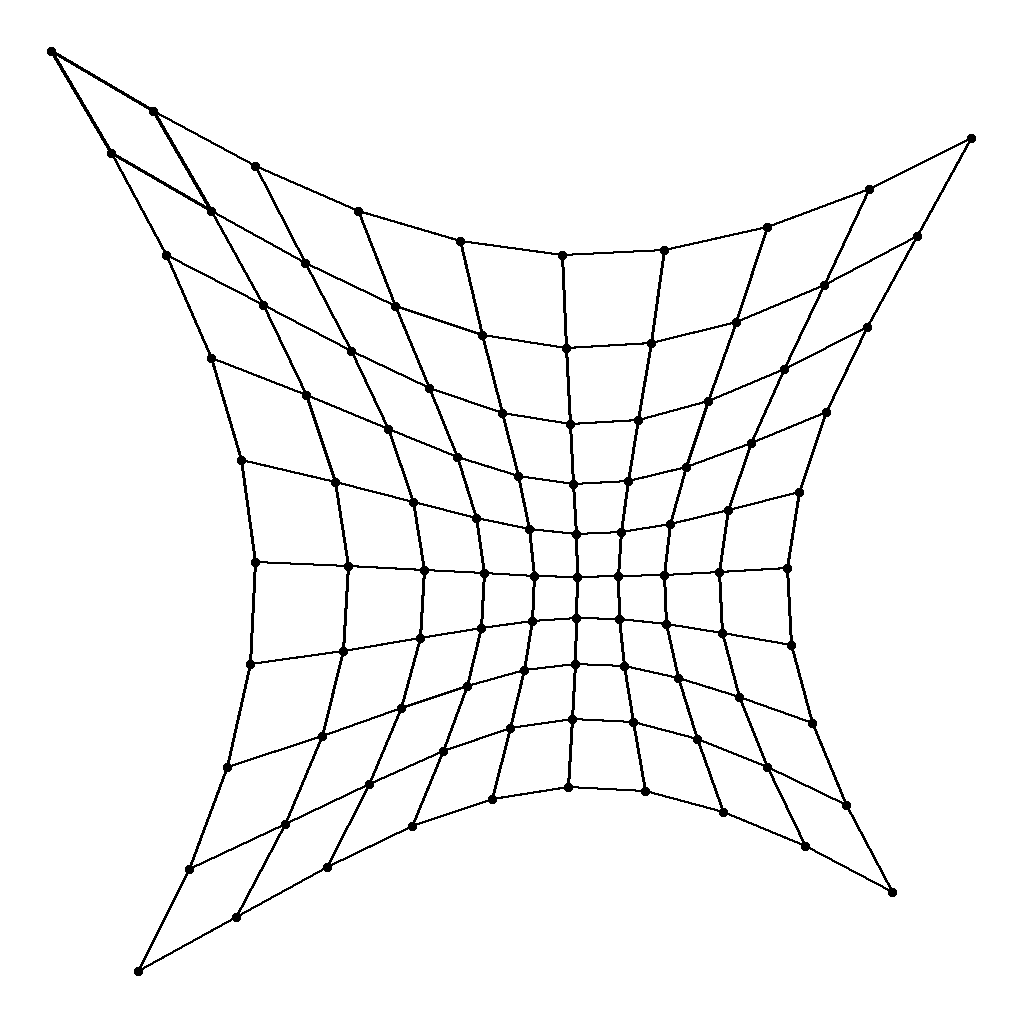
\includegraphics[width=\textwidth]{images/ima3.png}
%\caption{Grille Transformée}
%\label{fig:trnlin_mesh}
%\end{subfigure}
%\caption{Transformation non linéaire}\label{fig:trnlin}
%\end{figure}
%
%Dans le cas d'une application différentiable en un point, on peut d'une certaine façon faire coïncider localement la transformation non linéaire et l'endomorphisme qui lui est tangent en un point. Ceci est représenté sur la figure \ref{fig:diffapprox} où l'on remarque une très bonne coïncidence au voisinage du point où la différentielle est calculée.
%
%\begin{figure}[ht]
%\centering
%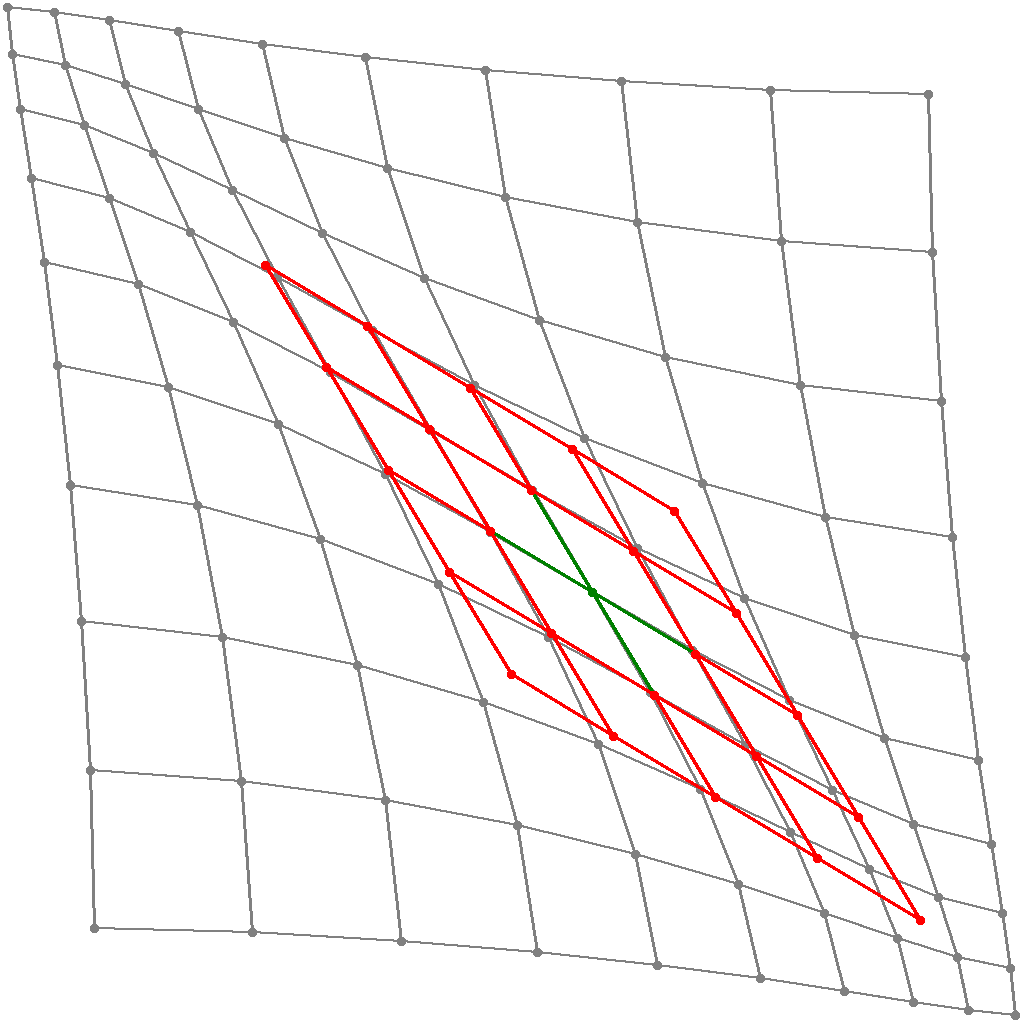
\includegraphics[width=0.5\textwidth]{images/ima4.png}
%\caption{Approximation par une application affine}\label{fig:diffapprox}
%\end{figure}
%
\subsection{Inversion locale}

\begin{fdefn}\label{def:diffeo}
Soient $U$ et $V$ deux ouverts de $\R^2$. On dit que $f \colon U \to V$ est un difféomorphisme de classe $C^1$ (ou $C^1$-difféomorphisme) 
si $f$ est bijective, de classe $C^1$ et si en outre l'application réciproque $g=f^{-1} \colon V \to U$ est de classe $C^1$
\end{fdefn}

\emph{Attention} : une application de classe $C^1$ peut être un homéomorphisme sans être un difféomorphisme de classe $C^1$ ; autrement dit l'application réciproque n'est pas nécessairement de classe $C^1$.

Il résulte du théorème de différentiation des applications composées que pour tout point $a \in U$ et $b=f(a)$, on a $g^\prime(b) \circ f^\prime(a)=f^\prime(a) \circ g^\prime(b) = \text{Id}_{\R^2}$ de sorte que les applications linéaires $g^\prime(b)$ et $f^\prime(a)$ sont inverses l'une de l'autre, donc des isomorphismes d'espaces vectoriels. En fait,nous avons un résultat plus fort :

\begin{fprop}
  \label{prop:homeo_diffeo}
   Soient $U$ et $V$ deux ouverts de $\R^2$, et $f \colon U \to V$ un homéomorphisme de classe $C^1$. Pour que $f$ soit un difféomorphisme de classe $C^1$, il faut et il suffit que, pour tout $x \in U$, $f^\prime(x)$ soit un isomorphisme d'espaces vectoriels.
\end{fprop}

Il est possible de s'affranchir de l'hypothèse imposant à $f$ d'être un homéomorphisme sous réserve de raisonner localement et 
d'introduire une notion de différentiabilité plus forte.

% \begin{fthm}
% Soit $U$ un  ouvert de $\R^2$ et soit $f \colon U \to \R^2$ une application de classe $C^1$. Supposons que, en un point $a \in U$, l'application dérivée $f^\prime(a)$ est un isomorphisme. Alors il existe un voisinage ouvert $W$ de $a$ ($W \subset U$) et un voisinage ouvert $V$ de $b=f(a)$, tels que $f$ soit un $C^1$-difféomorphisme de $W$ sur $V$.
% \end{fthm}
% Les propriétés de l'application linéaire tangente ne reflètent pas toujours celles de l'application initiale:
%   l'application $x \in \R \mapsto x^3$ est inversible sur $\R$ tout entier,
%   mais que sa dérivée en 0 est 0, donc non inversible. 
%   Pour obtenir une meilleure adéquation entre le comportement de l'application et de son modèle local, 
%   on imposera souvent une condition plus forte que la différentiabilité simple. 

\begin{fdefn}\label{def:strict_diff}
Soit $f \colon \Omega \to \R^2$. On dira que $f$ est strictement différentiable en $x_0 \in \Omega$ si l'on peut trouver un voisinage $V$ de $x_0$ et une application linéaire $H$ tels que:
\[
\forall (x,y) \in V^2, \, f(y) = f(x) + H(y-x) + o_{x_0}\left(\|y-x\|\right)
\]
\end{fdefn}

La différentiabilité stricte implique la différentiabilité simple, il suffit pour cela de considérer des couples de la forme $(x,x_0)$, mais la réciproque est fausse. L'intérêt majeur d'introduire cette notion réside dans le théorème suivant, dit d'inversion locale.

\begin{fthm}
Soit $f \colon \Omega \to \R^2$ une application strictement différentiable en $x_0 \in \Omega$. 
Si $f^\prime(x_0)$ est inversible, alors il existe un voisinage ouvert $U$ de $x_0$ et un voisinage ouvert $W$ de $f(x_0)$ 
tels que $f$ soit un homéomorphisme de $U$ sur $W$. De plus, $f^{-1}$ est strictement dérivable en $f(x_0)$ et on 
a $\left( f^{-1} \right)^\prime(f(x_0)) = \left(f^{\prime}\right)^{-1}(x_0)$.
\end{fthm}
La preuve est très classique. Elle est détaillée ci-dessous en raison de son caractère constructif qui fournit un algorithme numérique permettant d'inverser en un point une application. Un résultat intermédiaire fondamental, le théorème du point fixe, va être maintenant rappelé en préliminaire à la preuve proprement dite.

\begin{fthm} \label{thm:pt_fixe}
Soit $E$ un espace de Banach (i.e. espace vectoriel normé complet pour la topologie induite par la norme). Soit $f$ une application de $E$ dans $E$ telle qu'il existe un réel $1 > k > 0$ vérifiant:
\[
\forall (x,y) \in E, \, \|f(x)-f(y)\| \leq k \|x-y\|
\]
alors il existe un unique $x_0 \in E$ tel que $f(x_0)=x_0$.
\end{fthm}
Une application vérifiant l'hypothèse de majoration ci-dessus est dite contractante. Il est important de bien noter que le réel $k$ doit être strictement inférieur à 1. 
\begin{proof}
Soit $x$ un point quelconque de $E$. On pose, pour tout entier $n$: $x_0 = x, x_{n+1}=f(x_n)$. Pour tout entier $n \geq 1$, on a:
\[
\left\| x_{n+1}-x_n \right \| = \left\| f(x_n)-f(x_{n-1}) \right \| \leq k \left\| x_n-x_{n-1} \right \|
\leq k^n \left\| x_1-x_0 \right \| 
\]
on en déduit que pour tout couple d'entiers $1 \leq p < q$:
\[
\left\| x_q - x_p \right \| \leq \sum_{i=p}^{q-1} \left\| x_{i+1} - x_i \right \| \leq \sum_{i=p}^{q-1} k^i \left\| x_1-x_0 \right \| \leq \frac{k^p}{1-k} \left\| x_1-x_0 \right \|
\]
Prouvant ainsi que la suite $(x_n)_{n \in \N}$ est de Cauchy. Comme $E$ est un espace complet, elle admet une limite $x^*$ dans $E$. $f$ est Lipschitzienne, donc continue. On a ainsi:
\[
x^* = \lim_{n \to +\infty } x_{n+1} = \lim_{n \to +\infty} f(x_n) = f\left( \lim_{n \to +\infty} x_n \right)
=f(x^*)
\]
montrant que $x^*$ est un point fixe de $f$. L'unicité s'obtient facilement en supposant l'existence de deux points fixes distincts $x^*, x^{*\prime}$. La majoration vérifiée par $f$ donne:
\[
\|x^* - x^{*\prime}\|= \|f(x^*) - f(x^{*\prime})\| \leq k \|x^* - x^{*\prime}\|
\] 
ce qui est impossible car $k < 1$.
\end{proof}
\begin{rem}
Le théorème du point fixe présente deux aspects remarquables: 
\begin{itemize}
\item La convergence a lieu indépendamment du point de départ. 
\item La suite d'approximation du point fixe donne un algorithme explicite de calcul.
\end{itemize}
\end{rem}
On peut maintenant revenir à la preuve du théorème d'inversion locale qui sera, elle aussi, constructive.
\begin{proof}
L'idée principale est d'utiliser pour l'inversion le modèle linéaire fourni par la différentielle en $x_0$ en lieu et place de l'application $f$. 
Soit $V$ un voisinage de $x_0$ dans lequel l'application $f$ vérifie la condition de stricte différentiabilité:
\[
\forall (p,q) \in V, \, f(p)=f(q) +Df(x_0)(p-q) + o_{x_0}\left(\|p-q\|\right)
\]
avec~:
\[
 \left\|o_{x_0}\left(\|p-q\|\right)\right\| \leq \frac{\|Df(x_0)\|}{2} \|p-q\|
\]
Soit $y \in f(V)$. On pose, pour tout $x \in V$:
\[
\Theta_y(x) = x + Df^{-1}(x_0)\left(y-f(x)\right)
\]
On notera que $\Theta_y$ modifie $x$ de telle façon que l'on aurait $y=f(\Theta_y(x))$ si $f$ était une application affine. On espère ici que le modèle linéaire donné par la différentielle sera suffisamment bon pour que $f(\Theta_y(x))$ soit plus proche de $y$ que ne l'était $x$. L'application $\Theta_y$ est contractante. Pour tout couple $(x,z)$ de points de $V$ on a:
\begin{align*}
\left\|\Theta_y(x) - \Theta_y(z)\right\| &  = \left\|z-x + Df^{-1}(x_0)\left(f(x)-f(z)\right) \right \| \\
& = \left\|Df^{-1}(x_0)\left( Df(x_0)(z-x) + f(x)-f(z)\right) \right \| \\
& \leq \|Df^{-1}(x_0)\|  \left\|o_{x_0}\left(\|z-x\|\right)\right\| \leq \frac{1}{2} \|z-x\|
\end{align*}
De plus, pour $x \in V$:
\begin{align*}
&\left\| \Theta_y(x) - x_0 \right \|  = \left \| x-x_0 + Df^{-1}(x_0)\left(y-f(x)\right) \right \| \\
& \leq \left \| x-x_0 + Df^{-1}(x_0)\left(f(x_0)-f(x) \right) \right \| + \left\| Df^{-1}(x_0)\left(y-f(x_0)\right)\right\| \\
& \leq \frac{\|x-x_0\|}{2} + \|Df^{-1}(x_0)\|\|y-f(x_0)\|
\end{align*}
d'où l'on déduit que si l'on choisi $x$ dans une boule $B(x_0,r) \subset V$, $\Theta_y(x)$ sera encore dans cette boule sous réserve que $y$ appartienne à la boule de centre $f(x_0)$ et de rayon $\eta=\|Df(x_0)\|r/2$. Sous ces conditions, le théorème du point fixe montre qu'il existe $z$ tel que $\Theta_y(z)=z$, qui équivaut à $f(z)=y$. En choisissant comme domaine de départ une boule ouverte $B(x_0,r\prime)$ contenue dans l'ouvert $B(x_0,r) \cap f^{-1}(B(f(x_0,\eta)))$, on assure que $f$ réalise une bijection sur $f(B(x_0,r\prime))$.

Soient $y,z$ deux points de $f(B(x_0,r\prime))$. En remarquant que:
\[
\Theta_y(f^{-1}(y))=f^{-1}(y), \Theta_z(f^{-1}(z))=f^{-1}(z)
\]
il vient:
\begin{align*}
& \|f^{-1}(y) - f^{-1}(z) \| \leq \\ &
\| \Theta_z(f^{-1}(z)) -\Theta_y(f^{-1}(z)) \| + \| \Theta_y(f^{-1}(z))-\Theta_y(f^{-1}(y)) \| \\
& \leq  \| \Theta_z(f^{-1}(z)) -\Theta_y(f^{-1}(z)) \|  + \frac{1}{2} \|f^{-1}(y) - f^{-1}(z) \|
\end{align*}
d où l'on tire:
\[
\frac{1}{2} \|f^{-1}(y) - f^{-1}(z) \| \leq  \| \Theta_z(f^{-1}(z)) -\Theta_y(f^{-1}(z)) \| 
\]
Comme:
\[
\| \Theta_z(f^{-1}(z)) -\Theta_y(f^{-1}(z)) \|  = \| Df^{-1}(x_0) (z-y) \| \leq \| Df^{-1}(x_0)\| \|(z-y) \| 
\]
on a:
\[
\|f^{-1}(y) - f^{-1}(z) \| \leq  2 \| Df^{-1}(x_0)\| \|(z-y) \| 
\]
prouvant le caractère lipschitzien de $f^{-1}$.

Enfin:
\begin{align*}
& \|f^{-1}(z)-f^{-1}(y) +Df^{-1}(x_0)(y-z)\| \leq \\
& \| Df^{-1}(x_0)\| \| y-z+Df(x_0)\left(
f^{-1}(z) - f^{-1}(y)\right) \|
\end{align*}
Le terme $y-z+Df(x_0)\left(f^{-1}(z) - f^{-1}(y)\right)$ est dans $o_{x_0}(\|f^{-1}(z)-f^{-1}(y)\|)$, mais aussi 
dans $o_{f(x_0)}(\|z-y\|)$, $f^{-1}$ étant lipschitzienne. On en déduit la stricte différentiabilité de $f^{-1}$, avec une différentielle en $f(x_0)$ égale à $Df^{-1}(x_0)$.
\end{proof}
% \begin{rem}
% Le théorème d'inversion locale est vrai dans le cadre beaucoup plus général des espaces de Banach.
% \end{rem}

La proposition suivante permet d'utiliser le théorème d'inversion locale dans le cadre des applications de classe $C^1(U)$,
 $U$ ouvert, qui sont plus aisées à caractériser.
\begin{fprop}
Une application de classe $C^1(U)$ est strictement différentiable en tout point de $U$.
\end{fprop}
\begin{proof}
Soit $x_0\in U$ et soit $\epsilon > 0$. Par continuité de $f^\prime$, il existe un voisinage $V_\epsilon$ de 
$x_0$ tel que pour tout $y$ dans $V_\epsilon$:
\[
\left\| f^{\prime}(y)-f^\prime(x_0) \right\| \leq \frac{\epsilon}{2} 
\]
Pour tout couple de points $(y,z)$ de $V_\epsilon$:
\begin{align*}
f(z)-f(y)-f^\prime(x_0)(z-y) & = \left(f(z)-f(y)-f^\prime(y)(z-y) \right)  \\
& + \left(f^\prime(y)-f^\prime(x_0)\right)(z-y)
\end{align*}
Le premier terme du membre de droite est dans $o(\|z-y\|)$ en vertu de la différentiabilité de $f$ et quitte à réduire $V_\epsilon$, 
on peut supposer dans perte de généralité qu'il est majoré par $\epsilon \|z-y\| /2$. 
Le second terme est majoré par la même quantité, on a donc:
\[
\left\|f(z)-f(y)-f^\prime(x_0)(z-y)\right \| \leq  \epsilon \|z-y\|
\]
montrant la stricte différentiabilité de $f$ en $x_0$.
\end{proof}
La proposition précédente est locale: on peut supposer la différentiabilité au voisinage de $x_0$ et la 
continuité de $f^\prime$ en ce point pour assurer la strict différentiabilité en $x_0$.



\subsection{Calcul différentiel en coordonnées cartésiennes}

Les définitions et résultats énoncés ci-dessus sont intrinsèques, car ils ne ne dépendent pas du choix 
d' une base de $\R^2$, et peuvent être étendus aux espaces de Banach (espaces vectoriels normés complets).
Cependant, le calcul explicite de l'application dérivée se fera presque toujours en utilisant des coordonnées, ce qui motive
la définition suivante. 

\begin{defn}
Soit une application $f \colon U \to \R^2$. Soit $a$ un point de $U$ et soit $v$ un vecteur de $\R^2$. L'application $t \mapsto f(a+t v)$ est définie sur un ouvert de $\R$ contenant l'origine et à valeurs dans $\R^2$. Nous dirons que $f$ est \textit{dérivable dans la direction} du vecteur $v$, si la limite 
\[\lim_{t \rightarrow 0, t \neq 0} \frac{f(a+tv)-f(a)}{t}\]
existe. Lorsqu'elle existe, cette limite est appelée \textit{dérivée directionnelle} de $f$ au point $a$ dans la direction du vecteur $v$, et notée $L_v f(a)$. Lorsque $f$ est différentiable en $a$, alors
\[L_v f(a)=f^\prime(a) \cdot v.\]
\end{defn}


Une application peut avoir des dérivées directionnelles dans toutes les directions, sans être pour autant différentiable au point considéré. L'exemple classique est l'application $f \colon \R^2 \to \R$ définie par
\[f(x,y) = \begin{cases} \frac{x(x^2-3 y^2)}{x^2 + y^2} & \text{si} (x,y) \neq (0,0) \\
0 &  \text{si} (x,y)= (0,0).
\end{cases}\]
En effet, pour tout vecteur $v=(v_x, v_y)$, nous obtenons que $D_v f(0,0) = f(v_x,v_y)$. Mais comme cette fonction n'est pas une forme linéaire, elle ne peut pas s'écrire sous la forme $f^\prime(0,0) \cdot v$, et donc $f$ n'est pas différentiable en l'origine. 

Soit $(x_1,x_2)$ un système de coordonnées cartésiennes sur $\R^2$ et soit $U$ un ouvert de $\R^2$. On note $(e_1, e_2)$ la base canonique de $\R^2$. Une application $f \colon U \to \R^2$ peut donc se noter comme une application de deux variables $(x_1,x_2) \mapsto f(x_1,x_2)$. La \textit{dérivée partielle} de $f$ par rapport à sa première variable, ou par rapport à $x_1$, au point $a$ est la dérivée directionnelle de $f$ au point $a$ dans la direction du vecteur $e_1$. Elle est notée  $f^\prime_{x_1} (a)$ ou $\partial_{x_1} f (a)$. De même, on définit la dérivée partielle de $f$ par rapport à sa seconde variable, ou par rapport à $x_2$, au point $a$, par la dérivée directionnelle de $f$ au point $a$ dans la direction du vecteur $e_2$. 

On dira qu'une dérivée partielle de $f$ existe sur un ouvert $U$, si elle existe en tout point de $U$. Pour dériver par rapport à une variable, on considère que toutes les autres sont des constantes et on dérive, comme on a l'habitude, par rapport à la variable qui nous intéresse.

\begin{prop}
Si l'application $f \colon U \to \R^2$ est différentiable au point $a=(a_1,a_2) \in U$, alors toutes les dérivées partielles de $f$ existent au point $a$ et pour tout $v = (v_1,v_2) \in \R^2$ on a
\[f^\prime (a) \cdot v = \partial_{x_1}f(a) v_1 + \partial_{x_2}f(a)v_2.\]
Autrement dit :
\[f^\prime (a) = \partial_{x_1}f(a) e^\ast_1 + \partial_{x_2}f(a)e^\ast_2.\]
où $(e_1^\ast, e_2^\ast)$ est la base duale de la base canonique. 
\end{prop}

Il importe de noter que $f^\prime_{x_1} (a)$ et $f^\prime_{x_2} (a)$ appartiennent à $\mathcal{L}(\R, \R^2)$. Or, en raison de l'isomorphisme canonique entre $\mathcal{L}(\R, \R^2)$ et $\R^2$ \footnote{L'isomorphisme consiste à associer à un vecteur $v \in \R^2$, l'application linéaire $\lambda \mapsto \lambda v$ de $\R$ dans $\R^2$.}, ces différentielles s'identifient à un vecteur de $\R^2$. Plus précisément, la fonction $f$ peut s'écrire comme le couple $f=(f_1,f_2)$ où les $f_i$ sont des fonctions de $U$ dans $\R$. Dans ce cas, les dérivées partielles s'identifient à des nombres réels qui ne sont autres que des dérivées classiques de fonctions réelles. On définit donc en chaque point $a \in U$ et pour $i=1,2$, un vecteur $(\partial_{x_1} f_i (a),\partial_{x_2} f_i (a)) \in \R^2$, appelé le gradient de $f_i$ en $a$ et noté $\nabla f(a)$.   

\begin{definition}	Soit $U \subset \R^2$ un ouvert et soit $f \colon U \to \R^2$ une application différentiable en $a$. On appelle \textit{matrice jacobienne} de $f$ en $a$ la matrice de l'application linéaire $f^\prime(a)$ dans les bases canoniques de $\R^2$ :
\[\text{Jac} f(a) = \left( \partial_{x_j} f_i(a) \right)_{1 \leq i,j \leq 2}= \begin{pmatrix} \partial_{x_1} f_1(a) &\partial_{x_2} f_1(a) \\ \partial_{x_1} f_2(a) &\partial_{x_2} f_2(a).
\end{pmatrix}\]
\end{definition}

La proposition suivante est souvent utilisée pour prouver la différentiabilité. 

\begin{fprop} Si les dérivées partielles $\partial_{x_i} f(x)$ existent en tout point $x=(x_1,x_2) \in U$ et
   si les applications $\partial_{x_i}f \colon U \to \mathcal{L}(\R, \R^2) \simeq \R^2$ sont continues au point $a$,
    alors $f$ est différentiable au point $a$.
\end{fprop}

\begin{fprop}
Soit $f \colon U \to \R^2$. Si les dérivées partielles de $f$ existent et sont continues, alors $f$ est de classe $C^1(U)$.
\end{fprop}


Toutes ces notions et notations s'étendent immédiatement aux fonctions $f \colon U \subset \R^n \to \R^m$. 
% Pour plus de détails, la définition des dérivées secondes et successives et le théorème des fonctions implicites, 
% le lecteur est prié de se reporter à \cite{cartan1977} par exemple. 

\section{Holomorphie}
\begin{fdefn}
Une fonction complexe $f$ est dite \textbf{holomorphe} en $z_0$ si le quotient
\[\frac{f(z) - f(z_0)}{z - z_0}\]
admet une limite quand $z \rightarrow z_0$. Cette limite, appelée dérivée complexe de $f$ en $z_0$, est notée $f^\prime(z_0)$. Ainsi
\[f^\prime(z_0) = \lim_{z \rightarrow z_0}\frac{f(z) - f(z_0)}{z - z_0}.\]  
\end{fdefn}

Une définition équivalente est :
\begin{fdefn}
Une fonction complexe $f$ est dite \textbf{holomorphe} en $z_0$ si il existe $a \in \C$ tel que :
\[f(z)=f(z_0) + a(z-z_0) + o(\|z-z_0\|_E),\] pour $z \in V$ voisinage ouvert de $z_0$.
\end{fdefn}



\begin{exem}
La fonction puissance $f(z)=z^m$ a pour dérivée en tout point $z$, la fonction $f^\prime (z)=m z^{m-1}$. \end{exem}
\begin{exem}
 La fonction $f(z)=\overline{z}$ n'est dérivable en aucun point $z$. En effet, pour $h \in \C$,
\[\frac{f(z + h) - f(z)}{h}= \frac{\overline{h}}{h}.\]
Si $h$ est réel, le quotient vaut $1$, alors que si $h$ est imaginaire, le quotient vaut $-1$ ; par conséquent ce quotient n'admet pas de limite quand $h \rightarrow 0$. 
\end{exem}

La définition de l'holomorphie signifie que la fonction $f(z)$ est tangente en $z_0$ à l' application $\C$-affine:
\begin{equation}
  \label{eq:app_c_tangente}
  g_{z_0} \colon z \mapsto f(z_0) + f^\prime(z_0)(z-z_0).
\end{equation} 
$g_{z_0}$ s'écrit comme une composition:
\begin{equation}
  g = T_{f(z_0)}\circ H_{f^\prime(z0)} \circ T_{z_0}^{-1}
\end{equation} 
où, pour $a \in \C$,  $T_a$ désigne la translation par $a$ et $H_a$ l'application $\C$-linéaire $z \mapsto H_a(z) = az.$ Cette dernière 
transformation est elle-même la composée d'une homothétie de rapport $\lvert a \rvert$ et d'une rotation de centre $0$ et d'angle $\theta$ 
si $a=\lvert a \rvert e^{i \theta} .$ 
On en déduit que $g_{z_0}$ conserve les angles et multiplie les longueurs par un facteur $\lvert a \rvert.$
La même propriété est vérifié en $z_0$ par $f$ au sens suivant:


En particulier, l'angle de deux vecteurs attachés au point $z_0$ est conservé par une transformation holomorphe ainsi que le rapport
 des longueurs ; ceci n'est pas généralement le cas pour une fonction différentiable dans $\R^2$ (cf. Figure~\ref{fig:nonholo})

\begin{figure}[H]
\begin{center}
\shorthandoff{!}\shorthandoff{:}
\begin{tikzpicture}[line cap=round,line join=round,>=triangle 45,x=1.0cm,y=1.0cm, scale=0.22]
\clip(-15.093060716910394,0) rectangle (66.05423675849708,20);
\draw(10.,10.) circle (6.0229939275697255cm);
\draw [->,double distance=2pt,line width=0.5pt] (10.,10.) -- (14.450570388087627,5.941813327085688);
\draw [->] (10.,10.) -- (6.963521968330053,4.798437060389676);
\draw [->] (10.,10.) -- (9.059295023295197,15.949078079698115);
\draw [->,decorate,decoration={snake,amplitude=.4mm,segment length=2mm,post length=1mm}] (18,10) -- (25,10);
\draw [rotate around={43.337528513243676:(32.9136283378966,10.029232445533966)}] (32.9136283378966,10.029232445533966) ellipse (7.357654888453477cm and 3.919931190180329cm);
\draw [->,double distance=2pt,line width=0.5pt] (32.19368519771536,10.772399557979098) -- (38.84025582410203,13.922410528066017);
\draw [->] (32.19368519771536,10.772399557979098) -- (30.667497261883312,13.281485260282889);
\draw [->] (32.19368519771536,10.772399557979098) -- (30.438002710589707,4.309065433318341);
\begin{scriptsize}
\draw [color=black] (10.,10.) circle (5pt);
\draw[color=black] (10.59539099227846,10.84207147477083) node[font=\large] {$z$};
\draw [color=black] (32.19368519771536,10.772399557979098) circle (5pt);
\draw[color=black] (34,9.77376875063094) node[font=\large]  {$f(z)$};
\draw [fill=blue] (30.438002710589707,4.309065433318341) circle (2.5pt);
\end{scriptsize}
\end{tikzpicture}
\shorthandon{!}\shorthandoff{:}
\caption{Fonction différentiable mais non holomorphe : dilatation et rotation différentes pour des vecteurs attachés à un point de base $z$.}\label{fig:nonholo}
\end{center}
\end{figure}

\begin{rem}
Certains auteurs utilisent le mot \textit{analytic} (que l'on peut traduire en français par "analytique") pour désigner une fonction holomorphe. Nous parlerons de fonctions analytiques un peu plus loin par le prisme des séries entières.
\end{rem}

\subsection{Conditions de Cauchy-Riemann}
Soit $f \colon U \subset \C \to C$ une application différentiable en $z_0=x_0 +i y_0$. En écrivant $f=u + i v$, la dérivée $f^\prime (x_0,y_0)$ est une application linéaire de matrice jacobienne la matrice
\[\begin{pmatrix} \partial_x u &  \partial_y u \\ \partial_x v &  \partial_y v \end{pmatrix} \]
qui se décompose en la somme d'une application $\C$-linéaire et $\C$-antilinéaire. Pour être holomorphe, la partie antilinéaire de sa dérivée doit s'annuler. D'après la propiété \ref{prop:endomorphisme_c}, cela implique une matrice jacobienne de la forme suivante : $\begin{pmatrix} a &  -b  \\ b &  a \end{pmatrix}$. Ceci conduit aux conditions dites de Cauchy-Riemann $\partial_x u=\partial_y v$ et $\partial_y u=-\partial_x v$.

\begin{fprop}\label{prop:hol_1}
Pour que $f=u + i v$ soit holomorphe en $z_0$, il faut et il suffit que~:
\begin{MYenumerate}
\item $f$ soit différentiable en $z_0$ en tant qu'application de $\mathbb{R}^2$ dans $\mathbb{R}^2$ ;
\item $f$ satisfait aux conditions de Cauchy-Riemann~:
\[\begin{cases}
\partial_x u(z_0) &= \partial_y v(z_0)  \\
\partial_y u(z_0) &= - \partial_x v(z_0).
\end{cases}\]
\end{MYenumerate}
Dans ce cas, 
\[f^\prime(z_0)=\partial_x u(z_0) + i \partial_x v(z_0) = \partial_x f(z_0)=-i \partial_y f(z_0).  \]
\end{fprop}

\begin{fdefn}
Une application holomorphe en tout point d'un ouvert $U$ est dite holomorphe dans cet ouvert. L'ensemble des fonctions holomorphes dans $U$ sera notée $H(U)$.
\end{fdefn}


\paragraph{Opérateurs $\partial_z$ et $\partial_{\bar{z}}$} :  Nous introduisons les deux opérateurs différentiels suivants :
\[\partial_z = \frac{1}{2} \left(\partial_x -i \partial_y \right), \qquad \partial_{\bar{z}} = \frac{1}{2} \left(\partial_x + i \partial_y \right),\]
qui seront plus adaptés au calcul différentiel dans $\C$ que les classiques opérateurs $\partial_x$ et $\partial_y$. 

Ces opérateurs peuvent s'interpréter comme la dérivation par rapport aux variables $z$ et $\bar{z}$ respectivement, puisque 
\[\partial_z z=1, \; \partial_z \bar{z}=0, \; \text{ et } \;  \partial_{\bar{z}} z=0, \;\partial_{\bar{z}}\bar{z}=1.\]

Nous avons vu que si $f \colon U \to \C$ est différentiable en tant qu'application de $\R^2$ dans lui-même, alors
\begin{align*}
f(z)  = f(z_0) &+ \frac{1}{2} \left[(\partial_x u(z_0)-i \partial_y u(z_0)) + (\partial_x v(z_0) + i \partial_y v(z_0))\right](z-z_0) \\  &+  \frac{1}{2} \left[(\partial_x u(z_0) + i \partial_y u(z_0)) + (- \partial_y v(z_0) + i \partial_x v(z_0))\right]\overline{(z-z_0)} + o(\lvert z-z_0 \rvert) \\
=f(z_0) &+ \partial_z f(z_0) (z-z_0) + \partial_{\bar{z}} f(z_0) \overline{(z-z_0)} + o(\lvert z-z_0 \rvert).
\end{align*}
Cette expression traduit que lorsque $f$ est différentiable en $z_0$ en tant qu'application dans $\R^2$, son application dérivée est la somme de l'application $\C$-linéaire $\partial_z f(z_0)$ et de l'application $\C$-antilinéaire $ \partial_{\bar{z}} f(z_0)$. Ceci permet de reformuler la proposition \ref{prop:hol_1}:
\begin{fprop}
Pour que $f$ soit holomorphe en $z_0$, il faut et il suffit que :
\begin{MYenumerate}
\item $f$ soit différentiable en $z_0$ en tant qu'application de $\mathbb{R}^2$ dans $\mathbb{R}^2$ ;
\item $ \partial_{\bar{z}}f(z_0)=0$.
\end{MYenumerate}
Dans ce cas, $f^\prime(z_0)=\partial_z f(z_0)$.
\end{fprop}

Dans certains cas, il est nettement
plus simple de vérifier les conditions d'holomorphie à partir de cette forme. Il
suffit en effet de considérer dans l'expression de $f$ les variables
$z$ et $\overline{z}$ comme indépendantes et de calculer les dérivées partielles
correspondantes : si le terme antilinéaire est nul, la dérivée partielle par
rapport à $z$ donne directement $f^\prime(z_0)$.

\begin{exem} Soit $f(z)=\lvert z\rvert^2$, alors $\partial_z f(z)=\bar{z}$ et $ \partial_{\bar{z}} f(z)=z$, ainsi cette fonction n'est pas holomorphe. 

\end{exem}

La plupart des propriétés usuelles de la dérivation des fonctions de la variable réelle passent au cas complexe. 
\begin{fprop} 
Si $f \in H(U)$ et $g \in H(U)$, alors $f+g$ et $fg$ appartiennent aussi à $H(U)$ de sorte que $H(U)$ est un anneau auquel les règles usuelles de différentiation s'appliquent. 

La composée de deux fonctions holomorphes est holomorphe : si $f \in H(U)$, si $f(U) \subset U_1$, si $g \in H(U_1)$ et si $h=g \circ f$, alors $h \in H(U)$ et $h^\prime$ peut se calculer par la règle
\[h^\prime(z_0) =  g^\prime (f(z_0)) f^\prime (z_0), \quad (z_0 \in U).\]
  
Si $f \in H(U)$ et ne s'annule pas dans $U$, alors $(1/f) \in H(U)$ et : 
\[\left(\frac{1}{f}\right)^\prime (z_0)  = - \frac{f^\prime(z_0)}{f^2(z_0)}, \quad (z_0 \in U).\]
\end{fprop}

\begin{rem}[inversion locale]
Soit $\Omega$ un domaine de $\C$, et $f =u +i v$ holomorphe dans $\Omega$. Nous pouvons considérer $\Omega$ comme un domaine dans $\R^2$ et $f$ comme une application de $\Omega$ dans $\R^2$ de composantes $(u(x,y), v(x,y))$. Supposons $f  \in C^1(\Omega)$,  propriété qui ne découle pas, a priori, de l'holomorphie ; nous verrons ultérieurement qu'en fait si $f \in H(\Omega)$, alors $f \in C^\infty(\Omega)$. La matrice jacobienne de cette application est 
\[J_f=\begin{pmatrix}
\partial_x u & \partial_y u\\
\partial_x v &\partial_x v 
\end{pmatrix}\]
et le déterminant de cette matrice est
\[\det J_f=\partial_x u \partial_y v - \partial_y u \partial_x v.\]
L'utilisation des conditions de Cauchy-Riemann donne l'expression suivante~:
  \[\det J_f=(\partial_x u)^2 + (\partial_x v)^2=\lvert \partial_x u + i \partial_x v \rvert ^2.\]
Nous avons donc montré que si $f \in H(\Omega)$ alors le déterminant de sa matrice jacobienne (comme application de $\R^2$ dans $\R^2$) a pour déterminant $\det J_f(z)=\lvert f^\prime(z)\rvert^2$.

Nous pouvons donc utiliser le théorème d'inversion locale  pour obtenir :  soit $f \in H(\Omega)$, $z_0 \in \Omega$, et $f^\prime(z_0) \neq 0$, alors il existe un (petit) disque $U \subset \Omega$ contenant $z_0$ tel que $f(z)$ est bijective sur $U$, l'image $V=f(U)$ de $U$ est ouvert, et la fonction inverse 
\[ f^{-1} \colon V \to U\]
est holomorphe et satisfait
\[(f^{-1})^\prime (f(z))=1/f^\prime(z), \quad z \in U.\]
Notons que la propriété, importante, d'holomorphie de l'inverse ne découle pas du théorème d'inversion locale et doit être vérifiée.  
\end{rem}


\subsection{Fonctions harmoniques}

Soit $f$ une fonction de $\mathbb{R}^2 \to \mathbb{R}^2$. On dira que
$f$ est de classe $C^2$ dans un domaine $\Omega \subset \mathbb{R}^2$
si ses dérivées partielles secondes existent et sont continues dans
$\Omega$. Dans ce cas, on a $\partial_x \partial_y f= \partial_y \partial_x f$ et par conséquent
\[\partial_x^2 f + \partial_y^2 f=4 \partial_z  \partial_{\bar{z}}f.\]

C'est le laplacien de $f$, noté $\Delta f$. 

\begin{defn}
Une fonction $f$ de $\R^2$ dans $\R^2$ de classe $C^2$ est dite \textbf{harmonique} dans un domaine $\Omega$, si son laplacien est nul en tout point du domaine. 
\end{defn}

Soit $f \in H(\Omega)$ telle que les parties
réelle $u$ et imaginaire $v$ sont de classe $C^2$, alors du fait que $\partial_{\overline{z}} f =0$, ces applications réelles $u$ et $v$ sont harmoniques dans $\Omega$. En fait, nous verrons ultérieurement que lorsque $f=u + iv$ est holomorphe elle est nécessairement infiniment dérivable et donc $u$ et $v$ sont harmoniques. 

Si $u$ est une fonction réelle harmonique dans un domaine $\Omega$, et si $v$ est une fonction harmonique telle que la fonction $f=u + iv$ est holomorphe dans $\Omega$, nous dirons que $v$ est la fonction \textbf{harmonique conjuguée} de $u$. Cette fonction est unique, à une constante additive près, dans le sens où si $u + i v_0$ est aussi holomorphe, alors la différence $i(v-v_0)$ est holomorphe et $v-v_0$ est constante sur $\Omega$. Nous avons le résultat suivant~:   

\begin{theorem}
Soit $u(x,y)$ une application harmonique sur un domaine étoilé $\Omega$ de $\R^2$ dans un domaine étoilé $\Omega$ de $\mathbb{R}^2$. Alors, il existe une application harmonique $v(x,y)$ sur $\Omega$ telle que la fonction $f=u + iv$ est holomorphe sur $\Omega$. La fonction harmonique conjuguée est unique, à une constante additive près.   
\end{theorem}

La notion de fonction harmonique s'étend à toutes fonctions définies sur un ouvert de $\R^n$ ; ce sont les fonctions $f$ solution de l'équation, dite de Laplace, $\Delta f \equiv 0$, où $\Delta$ est l'opérateur laplacien $\sum_{i=1}^n \partial^2_{x_i^2}$. Ces fonctions jouent un rôle crucial dans de nombreux domaines tels que la physique, les mathématiques et les sciences de l'ingénieur. En particulier, les potentiels des principaux champs de vecteurs considérés en physique sont des fonctions harmoniques, et toute fonction harmonique, du point de vue de la physique, peut être représentée comme le potentiel d'un certain champ de vecteurs. C'est pour cette raison, que les fonctions harmoniques sont souvent appelées \textit{potentiels} et la théorie des fonctions harmoniques \textit{théorie du potentiel}. Ces fonctions jouissent de très nombreuses propriétés, qui sont partagées par les fonctions holomorphes ; pour plus de détails sur les fonctions harmoniques, se reporter à \cite{axler2013harmonic, rudin1988analyse}.

%\begin{proof}
%L'application $f$ recherchée sera de la forme~:
%$f = P + i Q$, différentiable en tout point de $\Omega$ et vérifiant
%les conditions de Cauchy. On pose~:
%\[
%\omega = - \frac{\partial P}{\partial y} dx + \frac{\partial P}{\partial
%  x} dy
%\]
%on a:
%\[
%d \omega = \left(\frac{\partial^2 P}{\partial x^2} + \frac{\partial^2
%P}{\partial y^2} \right)dx \wedge dy 
%\]
%Par hypothèse on a~:
%\[
%\frac{\partial^2 P}{\partial x^2} + \frac{\partial^2 P}{\partial y^2} = 0  
%\]
%on en déduite que $d\omega=0$. L'ouvert $\Omega$ étant étoilé, le théorème de Poincaré
%permet d'affirmer l'existence d'une application $Q$ (forme de degré 0, définie
%à une constante additive près) telle que $\omega = d Q$.
%En identifiant les expressions de $\omega$, on vérifie les conditions de Cauchy:
%\[
%\frac{\partial P}{\partial x} = \frac{\partial Q}{\partial y} ,\quad
%\frac{\partial P}{\partial y} = - \frac{\partial Q}{\partial x}
%\]
%montrant que $Q$ est bien la partie imaginaire recherchée.
%
%\end{proof}
%
\vspace*{1cm}

\begin{exercice}
Soit $\Omega$ un \textbf{domaine} non vide de $\mathbb{C}$ et soit $f \in H(\Omega)$. Montrer que les conditions suivantes sont équivalentes~:
%\renewcommand{\theenumi}{\alph{enumi}}
\begin{MYenumerate}
\item $f$ est constante sur $\Omega$ ;
\item $\text{Re}(f)$ est constante sur $\Omega$ ;
\item $\text{Im}(f)$ est constante sur $\Omega$ ;
\item $\lvert f \rvert$ est constante sur $\Omega$.
\end{MYenumerate}
\end{exercice}
\begin{exercice}
Soit $\Omega$ un ouvert de $\C$ ne contenant pas $0.$ Soit $f=P + i Q \colon \Omega \to \C$ une application $\R$ dérivable. Montrer, en posant $z=re^{i\theta}$ pour $z \in \Omega$, que les conditions de Cauchy en un point $z_0 = r_0 e^{i \theta_0}$ sont équivalentes à:
\[
\begin{cases}
    \frac{\partial P}{\partial r}\vert_{r_0,\theta_0} = \frac{1}{r}\frac{\partial Q}{\partial \theta}\vert_{r_0,\theta_0} \\
    \frac{\partial P}{\partial \theta}\vert_{r_0,\theta_0} =- r\frac{\partial Q}{\partial r}\vert_{r_0,\theta_0}
\end{cases}
\]
\end{exercice}
%\marginpar{
\includegraphics[scale=0.4]{images/k-word-icon.png}}


\section{Fonctions définies par des séries entières}
De nombreuses fonctions usuelles de la variable complexe s'obtiennent comme 
sommes de séries entières. Dans la suite du cours, nous verrons que cette
situation est générale pour des applications holomorphes dans un domaine de
$\mathbb{C}$. 

\subsection{Rayon de convergence}
Nous supposerons connu le résultat suivant~: 

\begin{fprop}\label{prop:ray_cvg}
\`{A} chaque série entière:
\[\sum_{n \geq 0} a_n (z-z_0)^n \quad (a_n \in \C)\]
correspond un nombre $R \in [0, \infty]$, tel que la série converge absolument et uniformément dans le disque fermé $\overline{B}(z_0 ; r)$, pour tout $r<R$, et diverge si $z \notin \overline{B}(z_0 ; R)$. Le \textbf{rayon de convergence} $R$ est donné par la formule de Cauchy-Hadamard 
\[\frac{1}{R}=\limsup_{n \to \infty} \lvert a_n\rvert^{\frac{1}{n}}.\]
\end{fprop}

\begin{proof}
Démontrons la convergence uniforme dans le disque fermé $\overline{B}(z_0 ; r)$, pour tout $r<R$ :
sans perte de généralité, on supposera $z_0 = 0$ pour simplifier l'écriture.
Soit $\alpha = \limsup_{n \to \infty } \lvert a_n\rvert^{\frac{1}{n}}$. Pour $z$ tel que $\lvert z\rvert < \frac{1}{\alpha}$, alors par continuité il existe $\epsilon > 0$ tel que $\lvert z\rvert < \frac{1}{\alpha +  \epsilon}$.

Par définition de la limite supérieure, il existe $N_\epsilon$ tel que pour $n \geq N_\epsilon, \lvert a_n \rvert^\frac{1}{n} < \alpha + \frac{\epsilon}{2}$, et donc $\lvert a_n z^n \rvert < \frac{\alpha + \frac{\epsilon}{2}}{\alpha + \epsilon}$, ce dernier terme, indépendant de $z$, étant celui d'une suite géométrique convergente.
\end{proof}

\begin{figure}[H]
\begin{center}
\shorthandoff{!}\shorthandoff{:}
\begin{tikzpicture}[line cap=round,line join=round,>=triangle 45,x=1.0cm,y=1.0cm]
\clip(-8,-2.3) rectangle (10,2.6);
\draw(0.,0.) circle (2.0084820138602186cm);
\draw(0.,0.) circle (1.6313184851524243cm);
\draw (0.,0.)-- (1.58,1.24);
\draw (0.,0.) node[anchor=north] {$z_0$};
\draw (0.4542148760330616,1.2748009015777618) node[anchor=north west] {$R$};
\draw (2.467738542449291,2.597114951164537) node[anchor=north west] {diverge};
\draw (2.6630803906837013,0.40845980465815337) node[anchor=north west] {converge};
\draw (2.2874229902329124,-0.6635912847483065) node[anchor=north west] {converge uniformément};
\draw (2.6480540946656697,1.5603005259203609) node[anchor=north west] {on ne sait pas};
\draw [->] (2.3775807663411017,2.2468519909842217) -- (1.476003005259208,2.2468519909842217);
\draw [->] (2.572922614575512,1.195011269722014) -- (1.8115098257343312,0.8674284704043167);
\draw [->] (2.6029752066115748,0.17322314049586957) -- (1.1454244928625135,0.17322314049586957);
\draw [->] (2.1371600300525966,0.17322314049586957) -- (1.8216078136739338,-0.11227648384672961);
\draw [->] (2.1822389181066915,-0.9988279489105902) -- (0.7096619083395983,-1.0138542449286219);

\end{tikzpicture}
\shorthandon{!}\shorthandoff{:}
\caption{Rayon de convergence d'une série entière.}
\end{center}
\end{figure}



\begin{fprop}(critère de Hadamard)
Le rayon de convergence $r$ d'une série entière $\sum_{n \geq 0} a_n z^n$ est
donné par:
\[
r^{-1}=\limsup_{n \to +\infty} |a_n|^{\frac{1}{n}}
\]
\end{fprop}
\begin{proof}
On suppose que: 
\[
0 < \alpha = \limsup_{n \to +\infty} |a_n|^{\frac{1}{n}} <
+\infty
\]
Si $|z|<\alpha^{-1}$, il existe $\epsilon > 0$ tel que $|z|\leq
(\alpha+\epsilon)^{-1}$. Par définition de la limite sup, il existe un entier
$N$ tel que pour tout $n \geq N$:
\[
|a_n|^{\frac{1}{n}} < \alpha + \frac{\epsilon}{2}
\]
et donc, pour tout $n \geq N$:
\[
\left|a_nz^n\right|< \left(\frac{\alpha + \frac{\epsilon}{2}}{\alpha +
\epsilon}\right)^n
\]
Le terme $|a_nz^n|$ est borné par le terme général d'une série géométrique
convergente, on  en déduit l'absolue convergence de la série entière.
De même, si $|z|> \alpha^{-1}$, le même raisonnement montre que le terme
$\left|a_nz^n\right|$ est divergent. Si $\alpha = +\infty$, il existe pour tout
réel $K>0$ et tout entier $N$ un entier $n$ tel que $|a_n|>K^n$, et donc aucun
rayon de convergence non nul ne peut exister pour la série entière. Enfin, si
$\alpha = 0$, pour tout $\epsilon > 0$, il existe un entier $N$ tel que pour
tout $n \geq N$, $|a_n|<\epsilon^n$: la série converge absolument dans tout
disque ouvert centré en 0.
\end{proof}
La formule de Cauchy-Hadamard n'est pas d'un emploi très aisé pour calculer le rayon de convergence. Le critère de d'Alembert ci-dessous est le plus couramment employé pour déterminer le rayon de
convergence ; il n'est néanmoins pas équivalent au critère de Cauchy-Hadamard.
\begin{fprop}
Soit $\sum_{n \geq 0}a_n (z-z_0)^n$ une série entière. Si la limite
\[\frac{1}{R} = \lim_{n \to \infty}\frac{\lvert a_{n+1}\rvert}{ \lvert a_{n} \rvert}
\]
existe, alors $R$ est le rayon de convergence de la série.
\end{fprop} 
Les opérations usuelles de combinaison linéaire et produit sont définies pour les séries entières convergentes.
\begin{fprop}
Soient $f \colon \sum_{n \neq 0}a_n(z-z_0)^n$ et $g \colon \sum_{n \geq 0} b_n (z-z_0)^n$ deux séries entières de rayons de convergence respectifs $r_1,r_2$. Pour tout $\lambda \in \C$, la série entière:
\[
h \colon z \mapsto \sum_{n \geq 0} (\lambda a_n + b_n) (z-z_0)^n
\]
a un rayon de convergence $r$ supérieur ou égal à $\inf(r_1,r_2)$. De plus, pour tout $z \in D(z_0,r), \, h(z) = \lambda f(z) + g(z)$.
\end{fprop}
\begin{proof}
Soit $z \in D(z_0, \inf(r_1,r_2)$. Pour tout $p \in \N$, on a:
\[
\sum_{n=0}^p \lvert \lambda a_n + b_n \lvert |z-z_0|^n \leq  \lvert \lambda\rvert  \sum_{n=0}^p \lvert a_n \lvert |z-z_0|^n + \sum_{n=0}^p \lvert b_n \lvert |z-z_0|^n 
\]
Les deux termes en partie de droite de l'inégalité ont une limite finie lorsque $p$ tend vers l'infini, prouvant ainsi que la série entière $h$ converge. La limite d'une série étant la limite de ses sommes partielles, on a immédiatement $h(z) = \lambda f(z) + g(z)$ par linéarité.
\end{proof}
\begin{fprop}
Soient $f \colon \sum_{n \neq 0}a_n(z-z_0)^n$ et $g \colon \sum_{n \geq 0} b_n (z-z_0)^n$ deux séries entières de rayons de convergence respectifs $r_1,r_2$. 
Pour tout $n \geq 0$, on pose:
\[
c_n = \sum_{k=0}^n a_k b_{n-k}
\]
La série entière:
\[
h \colon z \mapsto \sum_{n \geq 0} c_n (z-z_0)^n
\]
a un rayon de convergence $r$ supérieur ou égal à $\inf(r_1,r_2)$ et pour tout $z \in D(z_0,r), \, h(z) = f(z).g(z)$.
\end{fprop}
\begin{proof}
Soit $n \in N$. On a:
\[
\lvert \sum_{k=0}^n a_k b_{n-k} (z-z_0)^n\rvert \leq \sum_{k=0}^n \lvert a_k\rvert\lvert z- z_0\rvert^k \lvert b_{n-k}\rvert \lvert|z-z_0|^{n-k}
\]
On en déduit, pour $p \in \N$:
\[
\sum_{n = 0}^p  \sum_{k=0}^n \lvert a_k b_{n-k} (z-z_0)^n\rvert \leq \sum_{n=0}^p |a_n| |z-z_0|^n \sum_{m=0}^p |b_m||z-z_0|^m
\]
Par passage à la limite, on en déduit la convergence de la série $h$ si $|z-z_0| < \inf(r_1,r_2)$. L'écriture des sommes partielles donne directement $h(z)=f(z).g(z)$.
\end{proof}
\begin{fthm}
Soit $f$ une application définie par une série entière de rayon de
convergence $R$~:
\begin{equation}\label{eq:serie1}
f(z) = \sum_{n =0}^\infty a_n (z-z_0)^n,
\end{equation}
alors $f$ est holomorphe dans le disque ouvert $B(z_0 ; R)$ et l'on a~:
\begin{equation}\label{eq:serie2}
f^\prime(z) = \sum_{n = 1}^\infty n a_{n} (z-z_0)^{n-1}.
\end{equation}
\end{fthm}
\begin{proof}{(Preuve tirée de \cite{rudin1988analyse}).}
Selon le critère de Cauchy-Hadamard, si la série~(\ref{eq:serie1}) converge dans $B(z_0,r)$, alors la série~(\ref{eq:serie2}) y converge aussi. 
Prenons, $z_0=0$, sans perte de généralité, et notons par $g(z)$ la somme de la série~(\ref{eq:serie2}). Fixons $w \in B(0 ; R)$ et choisissons $r$ tel que $\lvert w \rvert < r <R$. Si $z \neq w$, alors
\[\frac{f(z) - f(w)}{z-w}-g(w)=\sum_{n=2}^\infty a_n \left[  \frac{z^n-w^n}{z-w} - n w^{n-1}\right].\]
L'expression entre crochets vaut
\[\sum_{k=1}^n w^{k-1}z^{n-k} - n w^{n-1} = (z-w) \sum_{k=1}^{n-1} k w^{k-1}z^{n-k-1}.\]
Si $\lvert z \rvert <r$, la valeur absolue de la somme précédente est inférieure à $\left(n(n-1)/2\right) r^{n-2}$
d'où
\[\Bigl | \frac{f(z) - f(w)}{z-w}-g(w) \Bigr |  \leq \lvert z-w \rvert \sum_{n=2}^\infty n^2 \lvert a_n \rvert r^{n-2}.\]
Comme $r<R$, la dernière série converge, donc le terme de gauche tend vers $0$ quand $z \to w$, d'où $f^\prime(w)=g(w)$. 
\end{proof}

Par récurrence immédiate, l'application $f$ sera indéfiniment dérivable dans son disque ouvert de convergence. Les coefficients de la série sont données par
\[a_n=\frac{1}{n!}f^{(n)}(z_0).\] 


\begin{rem}
Le rayon de convergence d'une série entière $\sum_{n=0}^\infty a_n z ^n$ est la distance du centre à la plus proche singularité (ce terme sera défini plus précisément au chapitre 5). Par exemple, le rayon de convergence de la série
$\sum_{n=0}^\infty z^n$ est $R=1$, puisque cette série ne converge pas en $z=1$. Notons que cette série représente la fonction $f(z)=1/(1-z)$, qui est définie pour tout $z \in \C \setminus \{1\}$ ; nous pouvons prolonger la fonction, définie par la série, à travers tous les points de la frontière du disque de convergence, sauf au point $z=1$. Le comportement sur le bord du disque de convergence peut être beaucoup plus compliqué. Considérons la série, dite lacunaire, $f(z)=\sum_n z^{2^n}$, exemple tiré de \cite{greene2006function} ; son rayon de convergence est $R=1$ car du fait que
\[\sum_n \lvert z^{2^n} \rvert < \sum_n \lvert z^{n} \rvert = \frac{1}{1-\lvert z \rvert},\]
nous en déduisons que cette série est absolument convergente pour tout $\lvert z \rvert <1$, et de plus elle diverge pour $z=1$.

Étudions la valeur de $f^\prime(z)$ au point $z=r \omega$ pour $0< r <1$ avec $\omega$ un point du cercle unité tel que $\omega^{2^N}=1$ pour un certain $N$. Alors
\begin{align*}
f^\prime(r \omega)&=\sum_{n=1}^{N-1} 2^n r^{2^n-1} \omega^{2^n-1} + \sum_{n=N}^{\infty} 2^n r^{2^n-1} \omega^{2^n-1} \\
&=\sum_{n=1}^{N-1} 2^n r^{2^n-1} \omega^{2^n-1} + \frac{1}{\omega}\sum_{n=N}^{\infty} 2^n r^{2^n-1} \cdot 1.
\end{align*}
Mais la série de droite diverge en $r=1$, donc $\lim_{r \to 1^-} \lvert f^\prime(r \omega) \rvert=\infty$ ; en outre l'ensemble des points $\omega$ satisfaisant les critères précédent est dense dans le cercle unité. Par conséquent, dans le voisinage de tout point du cercle unité, $f^\prime$ n'est pas bornée.

\end{rem}





\subsection{Fonctions analytiques}

\begin{fdefn}
On dit qu'une fonction $f$ définie dans un domaine (ou ouvert) $\Omega$ de $\mathbb{C}$, est \textbf{analytique} en $z_0 \in \Omega$, s'il existe un disque ouvert $B(z_0 ; r) \subset \Omega$ et une série entière
$\sum_{n \geq 0}a_n (z -z_0)^n$ de rayon de convergence supérieur $R>r$ tels que :
\[f(z) = \sum_{n =0}^\infty a_n(z-z_0)^n,\]
pour tout $z \in B(z_0 ; r)$. 

On dira que $f$ est \textbf{analytique} dans $\Omega$, si elle est analytique en tout
point de $\Omega$.
\end{fdefn}

Le fait d'être analytique est extrêmement contraignant pour une application ; elle doit au minimum être $C^\infty$, mais cela ne suffit pas. Par exemple, l'application
\[f \colon x \in \mathbb{R} \mapsto \left\{
\begin{array}{cc}
0 & \text{ si } x \notin ]-1,+1[ \\
\exp\left(\frac{-1}{1-x^2}\right) &  \text{ si } x \in ]-1,+1[
\end{array}
\right.
\]
est $C^\infty$, mais ne peut être analytique (ses dérivées aux points $-1,+1$
sont identiquement nulles).
En revanche, tout polynôme est analytique dans $\mathbb{C}$, car égal à son
développement en série de Taylor (qui est fini). 

De même, l'application $z
\mapsto z^{-1}$ est analytique dans $\mathbb{C}-\{0\}$. Soit $z \neq 0$, alors pour
tout $w \in \mathbb{C}$ tel que $|w|<|z|$, on peut écrire:
\[(z+w)^{-1}=  \frac{1}{z}\frac{1}{1+\frac{w}{z}} = \frac{1}{z} \sum_{n=0}^\infty (-1)^n \left( \frac{w}{z} \right)^n,\]
et le résultat est prouvé. 


L'exercice suivant permet de clarifier les points mentionnés ci-dessus.
\begin{exercice}
    Soit $\Omega$ un ouvert de $\C$ contenant l'origine et $f \colon \Omega \to \C$ une application développable en
    série entière au voisinage de $0$, de rayon de convergence $R > 0$. On dira que $z_0 \in \Omega$ est un point singulier de $f$ si $f$ n'est développable en série entière dans aucune boule ouverte de centre $z_0$ et de rayon non nul.
    \begin{itemize}
        \item Montrer qu'il ne peut exister aucun point singulier dans la boule ouverte $B(0,R).$
        \item Montrer qu'il existe au moins un point singulier sur $\partial B(0,R) = \Bar{B}(0,R)-B(0,R).$ 
    \end{itemize}
    Indice pour la deuxième question : on admettra la propriété suivante, qui est démontrée dans le chapitre sur les séries de Laurent : Une application holomorphe dans un domaine $\Omega$ est développable en série entière dans tout disque ouvert contenu dans $\Omega.$ 
     
\end{exercice}

\paragraph{Développement en série au point à l'infini.} Nous dirons qu'une fonction $f$ est analytique en $z_0=\infty$, si $g(z)=f(1/z)$ est analytique en $=0$. Ceci revient à considérer la fonction sur le plan complexe étendu $\overline{\C}$ ou encore sur la sphère de Riemann. Donc si $f$ est analytique en $\infty$, alors $g(z)$ admet le développement en série entière $g(z)=\sum_{n=0}^\infty a_n z^n$, pour $\lvert z \rvert <\rho$, où $\rho$ est le rayon de convergence de cette série. Par conséquent, $f$ admet le développement en puissance de $z$ suivant :
\[f(z)=\sum_{n=0}^\infty \frac{a_n}{z^n}, \qquad \lvert z \rvert > \frac{1}{\rho}.\]
Cette série converge absolument pour $\lvert z \rvert > \frac{1}{\rho}$ et pour tout $r>1/ \rho$, cette série converge uniformément pour $\lvert z \rvert \geq r$.

\begin{exem} Si $n \geq 0$, la fonction $f(z)=1/z^n$ est analytique en $z=\infty$, car $g(w)=w^n$ est analytique en $w=0$. 
\end{exem}


\paragraph{Les zéros d'une fonction analytique}
Soit $f$ une fonction analytique en $z_0$, et supposons que $f(z_0)=0$ mais que $f(z)$ ne soit pas identiquement nulle. Nous dirons que $f(z)$ a un \textbf{zéro d'ordre $N$}  en $z_0$, si $f(z_0)=f^\prime(z_0) = \cdots = f^{(N-1)}(z_0)=0$ et $f^{(N)}(z_0) \neq 0$. Le développement en série entière de $f$ en $z_0$ a la forme suivante : 
\[f(z)=a_N(z-z_0)^N + a_{N+1} (z-z_0)^{N+1} + \cdots,\]
avec $a_N \neq 0$. Nous pouvons mettre le terme $(z-z_0)^N$ en facteur et écrire 
\[f(z)=(z-z_0)^N h(z)\]
avec $h(z)$ analytique en $z_0$ et $h(z_0)\neq 0$. 

Nous dirons qu'un point$z_0 \in E$ est un \textbf{point isolé} de l'ensemble $E \subset \C$, s'il existe un $\rho>0$ tel que $\lvert z-z_0\rvert  \geq \rho$ pour tout autre point $z \in E$. En d'autre termes, $z_0$ est un point isolé de $E$, s'il est à une distance non nulle de tout point de $E \setminus \{z_0\}$. Si $E$ est un ensemble tel que chaque point de $E$ est un point isolé de $E$, nous dirons que les points de $E$ sont isolés. 

\begin{exem} Si $E=[-1,0] \bigcup \{1/n : n \geq 1\}$, chacun des points $1/n$ sont isolés dans $E$, à la différence des points de l'intervalle $[-1,0]$ qui ne le sont pas.
\end{exem}

Une conséquence importante de l'analycité est le résultat suivant connu sous le nom du théorème des zéros isolés :
\begin{fthm}(Théorème des zéros isolés)
Si $f$ est une application analytique non identiquement nulle dans un domaine
$\Omega$, alors les zéros de $f$ sont des points isolés.
\end{fthm}
\begin{proof}
La difficulté majeure du théorème vient de son caractère global. On va tout
d'abord prouver un résultat local au voisinage d'un zéro, puis conclure grâce à la connexité du domaine. 

Soit $z_0 \in \Omega$ un zéro d'ordre $N$ de $f$. Nous pouvons alors factoriser $f$ sous la forme $f(z)=(z-z_0)^N h(z)$, avec $h(z)$ une fonction analytique en $z_0$ telle que $h(z_0) \neq 0$. Alors pour $r>0$ suffisamment petit, nous avons $h(z) \neq 0$ pour tout $z \in B(z_0 ;r)$, d'où $f(z) \neq 0$ pour $0 < \lvert z-z_0 \rvert <r$. Ainsi, $f$ n'admet pas d'autre zéro a une distance plus petite que $r$ de $z_0$, et donc $z_0$ est un point isolé.

Le passage au global se fait par un argument de connexité. Pour cela, considérons l'ensemble $\mathcal{O}$ des $z$ tels que $f^{(m)}(z)=0$ pour tout $m \geq 0$ (c'est à dire l'ensemble des zéros non isolés).
\begin{itemize}
    \item[$\bullet$] Si $z_0 \in \mathcal{O}$, alors son développement en série $f(z)=\sum a_n (z-z_0)^n$ est tel que $a_n=f^{(n)}(z_0)/n!=0$ pour tout $n \geq 0$. Donc $f(z)=0$ pour tout $z$ dans un disque centré en $z_0$, et tous les points de ce disque appartiennent à $\mathcal{O}$. Ceci prouve que $\mathcal{O}$ est ouvert dans $\Omega$.
    \item[$\bullet$] Si $z_0 \in \Omega \setminus \mathcal{O}$, alors il existe un $n$ tel que $f^{(n)}(z_0) \neq 0$, d'où par continuité $f^{(n)}(z) \neq 0$ dans un disque centré en $z_0$. Ce disque est donc contenu dans $\Omega \setminus \mathcal{O}$, ce qui implique que $\mathcal{O}$ est fermé dans $\Omega$.
\end{itemize}
Comme par hypothèse $\Omega$ est connexe, nous avons soit $\mathcal{O}=\Omega$, soit $\mathcal{O}$ est vide (sinon $\Omega$ serait la réunion des deux ouverts disjoints $\mathcal{O}$ et son complémentaire dans $\Omega$). Nous avons supposé $f$ non identiquement nulle, donc $\mathcal{O}=\emptyset$. Nous en concluons que tous les zéros de $f$ sont d'ordre fini.
\end{proof}

\begin{rem}
Attention, le théorème des zéros isolés n'exclut pas l'existence de zéros non isolés dans $\C \setminus \Omega$ ; en particulier , une application analytique non constante sur un ouvert $U$ peut avoir des zéros s'accumulant sur la frontière $\partial U$. Par ex. la fonction $f(z)=\sin(1/(1-z))$ sur le disque unité (la fonction $\sin(z)$ est décrite ci-dessous) admet pour zéros les points $1-(n\pi)^{-1}$ qui s'accumulent sur le point frontière $1$. 
\end{rem}


\begin{fprop}
Soit $f$ analytique dans un domaine $\Omega$. Le développement en série entière
de $f$ au voisinage de chaque point de $\Omega$ est unique.
\end{fprop}


%On notera également que l'ensemble des zéros de $f$ dans un compact $K$ donné ne
%peut être que de cardinal fini si $f$ n'est pas identiquement nulle.

En appliquant le théorème des zéros isolés à $f(z)-g(z)$, nous obtenons le résultat suivant, d'un usage important~:
\begin{fprop}(Prolongement analytique) \label{prop:prolongement}
Si deux applications $f$ et $g$ sont analytiques dans un domaine $\Omega$ et si $f(z)=g(z)$ pour tout $z$ appartenant à un ensemble ayant un point non isolé, alors $f(z)=g(z)$ pour tout $z \in \Omega$.
\end{fprop}




 
\section{Fonctions élémentaires}

Un grand nombre d'applications réelles usuelles s'étendent en une fonction analytique définie sur $\C$, nous en verrons les plus classiques dans la suite. Ce prolongement à $\C$ ne peut se faire que d'une seule façon puisque par application de la proposition~\ref{prop:prolongement}, si $f$ et $g$ sont des fonctions analytiques sur $\C$ et si $f(x)=g(x)$ pour tout $x \in \R$, alors $f=g$. Une fonction analytique définie sur $\C$ est dite \textbf{fonction entière}.

Nous verrons que des fonctions apparemment différentes, lorsque considérées comme des fonctions réelles, présentent en fait des relations lorsqu'elles sont vues comme des fonctions définies sur $\C$. Citons à ce propos Paul Painlevé (1863-1933) \og \emph{entre deux vérités du domaine réel, le chemin le plus facile et le plus court passe bien souvent par le plan complexe}\fg{}.

\subsection{Fonction exponentielle}
C'est l'application entière, notée $e^z$ et
définie par la série entière de rayon de convergence infini~:
\[
e^z = \sum_{n= 0}^\infty \frac{z^n}{n!}.\]
Pour les $z=x$ réels cette fonction coïncide avec la définition ordinaire de l'exponentielle.

La formule connue de dérivation est conservée : 
\[(e^z)^\prime=e^z.\]
 
La propriété fondamentale de l'exponentielle est conservée : pour $z_1,z_2 \in \mathbb{C}$, on a
\[e^{z_1+z_2} = e^{z_1} e^{z_2}.\]
Ceci découle des calculs suivants :
\begin{align*}
e^{z_1+z_2} & = \sum_{n \geq 0} \frac{(z_1+z_2)^n}{n!} = 
\sum_{n \geq 0} \frac{1}{n!}\sum_{k=0}^n \binom{n}{k} z_1^k z_2^{n-k} \\
& = \sum_{n \geq 0} \sum_{k=0}^n \frac{z_1^k}{k!} \frac{z_2^{n-k}}{(n-k)!} = \Bigl(\sum_{k=0}^\infty  \frac{z_1^k}{k!}\Bigr)\Bigl(\sum_{m=0}^\infty  \frac{z_2^m}{m!}\Bigr)\\
&=e^{z_1} e^{z_2}.
\end{align*}
On en déduit aisément que $e^{-z}=1/e^z$.

Considérons la fonction $f(y)=e^{iy}$ avec $y \in \R$; son développement en série entière en zéro est donné par :
\begin{align} \label{eq:exposerie}
e^{iy} &= 1+\frac{iy}{1!} +  \cdots + \frac{(iy)^n}{n!} + \cdots \\
&=1-\frac{y^2}{2!} + \frac{y^4}{4!} + \cdots + i \Bigl( y- \frac{y^3}{3!} + \frac{y^5}{5!} + \cdots \Bigr).
\end{align}
Nous reconnaissons dans le premier terme de droite le développement en série entière de la fonction $\cos y$ et dans le deuxième terme, le développement en série entière de la fonction $\sin y$. Nous en déduisons la formule connue
\[\exp^{x + i y} = e^x (\cos y + i \sin y).\]

\begin{figure}[hbt]
\begin{center}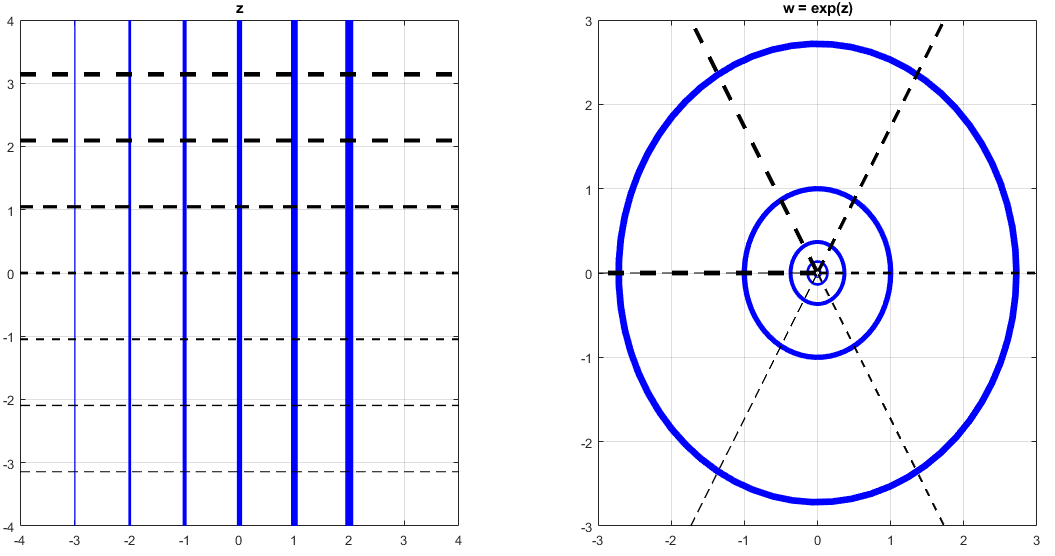
\includegraphics[scale=0.55]{images/complexexp3.png}
\end{center}
\caption{\small Fonction $f(z)=e^z$ : Les droites $y=y_0$ sont transformées en les rayons $\theta_0=y_0$ (on remarque que les images des droites $y=-\pi$ et $y=\pi$ se recouvrent) et les segments $x=x_0$, $0 \leq y < 2 \pi$, en les circonférences $r=e^{x_0}$.}\label{fig:expo}
\end{figure}
En particulier, la fonction exponentielle ne s'annule jamais, puisque $\lvert e^z\rvert = e^x$ qui n'est jamais nul. D'autre part, la fonction exponentielle d'une variable complexe possède aussi une propriété spécifique : elle est périodique de période purement imaginaire $2 \pi i$. En effet, pour tout entier $k$
\[e^{z + 2 k \pi i}=e^z e^{2 k \pi i}=e^z.\]

En vertu de cette périodicité, l'étude de la fonction $e^z$ dans tout le plan se ramène à son étude dans la bande $0 \leq y < 2 \pi$ (cf. figure~\ref{fig:expo}). 



\subsection{Fonctions trigonométriques et hyperboliques}
Les fonctions trigonométriques et hyperboliques s'expriment simplement à l'aide de la fonction exponentielle. Le développement en série~(\ref{eq:exposerie}) de $e^{i z}$ conduit à définir les fonctions trigonométriques
\[\cos z = \frac{1}{2}\left(e^{i z} + e^{-iz}\right), \quad \sin z=\frac{1}{2 i} \left(e^{i z} - e^{-iz}\right).\]
Ces fonctions coïncident pour $z=x$ réel aux fonctions trigonométriques réelles et sont analytiques dans tout le plan $\C$. Elles vérifient les formules ordinaires de dérivation :
\[(\sin z)^\prime=\cos z, \quad (\cos z)^\prime=-\sin z ;\]
sont périodiques de période réelle $2 \pi$ et vérifient les relations trigonométriques
\[\cos^2 z+\sin^2 z =1, \quad \sin 2 z = 2 \sin z \cos z.\]

% \begin{figure}[hbt]
% \begin{center}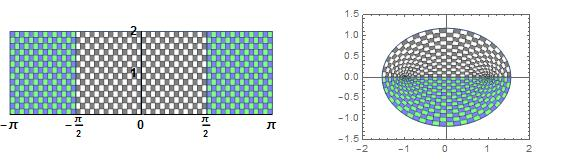
\includegraphics[scale=0.9]{sinus}
% \end{center}
% \caption{\small Image de la bande $\{-\pi \leq x < \pi, 0\leq y < 2\}$ par la fonction $f(z)=\sin z$. La familles des rayons $x=x_0$ et des segments $y=y_0$ se transforment respectivement en les familles des hyperboles et des ellipses homofocales ; la bande $-\pi/2 < x<\pi/2, y>0$ se transforme dans le demi-plan supérieur.}\label{fig:sin}
% \end{figure}

Nous voyons que dans le domaine complexe, $\cos$ et $\sin $ \textbf{ne sont pas bornées}. Par exemple pour $\sin$, si $x=\pm \pi/2$, $y>0$, elle prend  des valeurs réelles supérieures en module à l'unité et, en général, aussi grandes que l'on veut.

\begin{figure}[hbt]
\begin{center}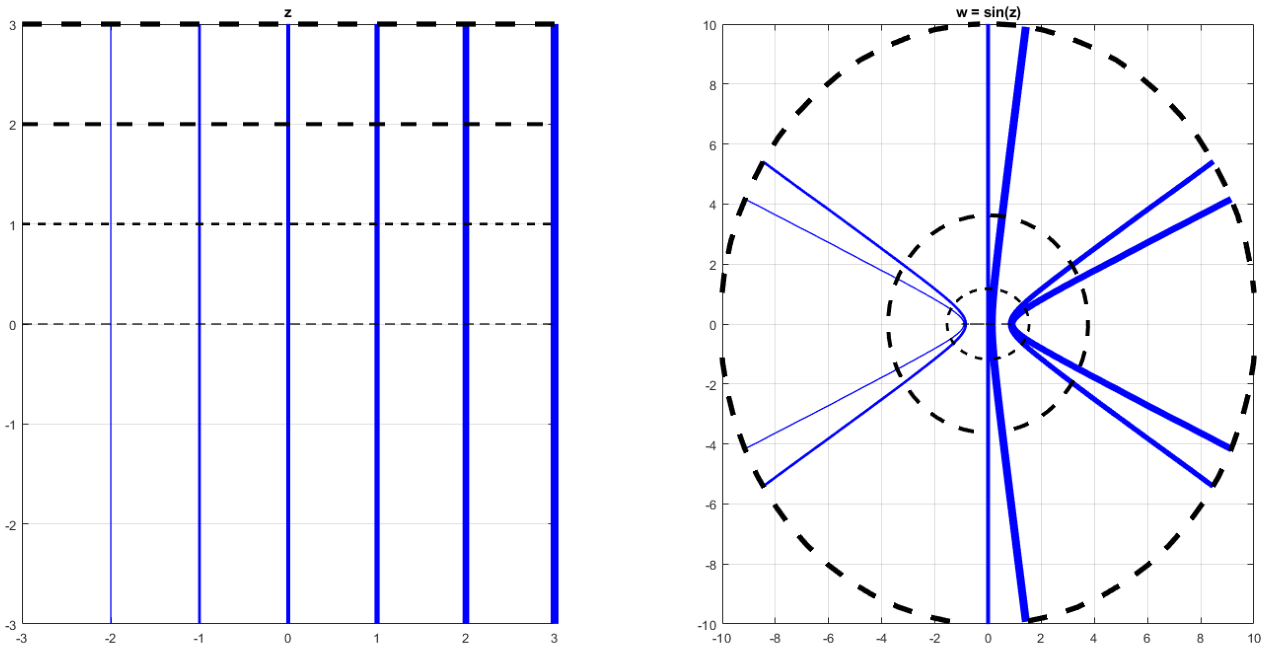
\includegraphics[scale=0.46]{images/complexsin3.png}
\end{center}
\caption{\small Image de droites par la fonction $f(z)=\sin z$. Les droites $x=x_0$ et $y=y_0$ se transforment respectivement en les familles des hyperboles et des ellipses homofocales ; la bande $-\pi/2 < x<\pi/2, y>0$ se transforme dans le demi-plan supérieur.}\label{fig:sin}
\end{figure}

Les fonctions $\tan z$ et $\cot z$ sont définies par les formules
\[\tan z= \frac{\sin z}{\cos z}, \quad \cot z =  \frac{\cos z}{\sin z}.\]
La fonction $\tan z$ est partout analytique excepté aux points annulant $\cos z$, c'est-à-dire aux points $z_k=\frac{\pi}{2} + k\pi$ ($k=0, \pm 1, \pm 2, \cdots$). Il en est de même de la fonction $\cot z$ et des points $z_k= k\pi$ ($k=0, \pm 1, \pm 2, \cdots$).

On a \[ (\tan z)' = \frac{1}{\cos^2 z} \]

Les \textbf{fonctions hyperboliques} dans le plan complexe sont définies par
\[\sh z= \frac{e^z-e^{-z}}{2}, \quad \ch z= \frac{e^z+e^{-z}}{2},\]
et
\[\th z=\frac{\sh z}{\ch z}, \quad \cth z=\frac{\ch z}{\sh z}.\]
Fait remarquable, ces fonctions s'expriment très simplement à l'aide des fonctions trigonométriques
\[\begin{cases}
\sh z= - i \sin iz, & \ch z=\cos iz,\\
\th z= -i \tan i z, & \cth z=i \cot iz.
\end{cases}\]

Ces fonctions vérifient les formules ordinaires : 
\[\ch ^2 z-\sh^2 z = 1, \quad (\ch z)^\prime= \sh z, \quad, (\sh z)^\prime=\ch z.\] 
$\ch$ et $\sh$ sont holomorphes dans $\C$, et $\th$ est holomorphe dans $\C \setminus \big\{ i\left( \frac{n+1}{2} \right) \pi \big\}$

\begin{exercice}
Montrer que 
\[\frac{e^z}{1+z}=1+\frac{1}{2}z^2 - \frac{1}{3}z^3 + \frac{3}{8}z^4 -\frac{11}{30}z^5 + \cdots.\]
Montrer que le terme général de la série est donné par
\[a_n=(-1)^n \left[\frac{1}{2!} - \frac{1}{3!} + \cdots + \frac{(-1)^n}{n!}\right], \quad n \geq 2.\]

Quel est le rayon de convergence de la série ?
\end{exercice}

\begin{exercice} \label{ex:log}
Soit la série entière :
\[f(z)= \sum_{n >0}(-1)^{n-1}\frac{(z-1)^n}{n}
\]
\begin{itemize}
  \item déterminer son rayon de convergence ;
  \item montrer que pour tout réel $x \in ]0,2[$, $f(x)=\log(x)$;
  \item en déduire que $f$ est l'unique application analytique prolongeant le
  logarithme réel sur le disque ouvert $B(1 ; 1)$;
  \item vérifier que pour tout $z \in B(1 ;1)$, on a $\exp^{f(z)}=z$.
\end{itemize}
\end{exercice}






\subsection{Fonction logarithme}

Nous introduisons dans cette partie, la fonction logarithme complexe, en suivant l'approche de \cite{remmert1991theory}. La difficulté réside dans le fait que la fonction exponentielle $e^z$ n'est pas injective, car étant périodique de période $2 i \pi$. Elle ne peut être bijective qu'en considérant, par exemple, la bande $\{ -\pi < y <\pi\}$. 

\begin{fdefn}
Une fonction analytique $\ell \colon  \Omega \to \C$, sur un domaine $\Omega \subset \C$, est appelée \textbf{fonction logarithme} sur $\Omega$ si $\exp(\ell( z)) = z$ pour tout $z \in \Omega$. 
\end{fdefn}
Si nous disposons d'une fonction logarithme $\ell$, alors toutes les autres s'en déduisent. Plus particulièrement,
\begin{prop}
Soit $\ell \colon \Omega \to \C$ une fonction logarithme sur $\Omega$. Les propositions suivantes concernant une fonction $\hat{\ell} \colon \Omega \to \C$ sont équivalentes :
\begin{MYenumerate}
\item $\hat{\ell}$ est une fonction logarithme sur $\Omega$ ;
\item $\hat{\ell} = \ell + 2 \pi i n$ pour un certain $n \in \Z$.
\end{MYenumerate}
\end{prop}

\begin{proof}
$i)\implies ii)$ Nous avons $\exp(\hat{\ell}(z))=\exp(\ell (z))$, d'où $\exp (\hat{\ell}(z)-\ell(z))=1$ pour tout $z \in \Omega$. Donc $\hat{\ell}(z)-\ell(z) \in 2 \pi i \Z$ pour tout $z \in \Omega$. La fonction $\frac{1}{2 \pi i}(\hat{\ell} -\ell)$ doit être continue et à valeurs entières sur un domaine, d'où constante et donc égale à un certain $n \in \Z$.

$ii) \implies i)$ $\hat{\ell}$ est analytique dans $\Omega$ et vérifie $\exp(\hat{\ell}(z))=\exp(\ell(z)) \exp(2 \pi i n)=\exp (\ell(z))=z$
pour tout $z \in \Omega$. n 
\end{proof}
Les fonctions logarithmes sont caractérisées par leur première dérivée

\begin{prop}
Les assertions suivantes sur une fonction $\ell$ analytique sur $\Omega$ sont équivalentes :
\begin{MYenumerate}
\item $\ell$ est une fonction logarithme sur $\Omega$ ;
\item $\ell^\prime(z)=1/z$ sur $\Omega$ et $\exp(\ell(a))=a$ pour au moins un $a \in \Omega$.
\end{MYenumerate}
\end{prop}

\begin{proof}
$i) \implies ii)$ Il suffit de dériver la relation $\exp(\ell(z))=z$ pour obtenir l'identité fonctionnelle $1=\ell^\prime(z) \exp (\ell(z))=\ell^\prime(z) z$ et donc $\ell^\prime(z)=1/z$.

$ii) \implies i)$ La fonction $g(z) := z \exp(-\ell(z))$, $z \in \Omega$, est analytique dans $\Omega$ et vérifie $g^\prime(z)=0$ pour tout $z \in \Omega$. Il s'ensuit que $g =c \in \C \setminus\{0\}$ ; d'où $c \exp(\ell(z))=z$ dans $\Omega$. Puisque $\exp(\ell(a))=a$, alors $c=1$.
\end{proof}

L'exercice~\ref{ex:log} montre l'existence d'une fonction logarithme sur $B(1;1)$, à savoir la fonction
\[\log z := \sum_{n=1}^\infty  \frac{(-1)^{n-1}}{n}(z-1)^n.\]
Il est alors aisé de transférer cette existence à tout autre disque $B(a ;\lvert a \rvert)$ avec $a \in \C^\ast$ en considérant la fonction $\ell_a(z) : =\log(z a^{-1}) + b,$ où $b$ est un logarithme de $a$. En effet,
\[\exp(\ell_a(z))=\exp(\log(z a^{-1})) \exp(b)=z a^{-1}a=z.\]

Nous pouvons construire une fonction logarithme dans $\Omega_0 := \C \setminus ]-\infty,0]$ qui est le plan $\C$ coupé selon l'axe des $x$ négatifs. Nous partons de la fonction réelle $\log \colon \R^+ \to \R$ qui à $r>0$ associe $\log r$. Nous prolongeons cette fonction à tout $z \in \Omega_0$, en prenant la représentation $z=\lvert z\rvert e^{i  \varphi}$ où $\lvert z\rvert>0$ et $-\pi< \varphi < \pi$. Nous avons

\begin{fprop}
La fonction $\log \colon  \Omega_0 \to \C$, $z=\lvert z\rvert e^{i  \varphi} \mapsto \log \lvert z\rvert + i \varphi$ ($-\pi< \varphi < \pi$) est une fonction logarithme sur $\Omega_0$. Dans $B(1 ; 1)$, elle coïncide avec la fonction définie par le développement en série $\sum_1^\infty \frac{(-1)^{n-1}}{n}(z-1)^n$. Cette fonction est appelée \textbf{détermination principale} du logarithme dans $\Omega_0$ et $\varphi$ l'\textbf{argument principal} de $z$.
\end{fprop}
\begin{proof}
La continuité de la fonction est prouvée grâce à un argument de compacité (sous suite convergent) et le fait que l'argument principal interdit deux arguments séparés de plus de $2 \pi$. Ensuite
\[\exp(\log z)=e^{\log \lvert z \rvert} e^{i \varphi}=  \lvert z \rvert e^{i \varphi}=z,\]
pour tout $z\in \Omega_0$. Par ailleurs, la fonction $\sum_1^\infty \frac{(-1)^{n-1}}{n}(z-1)^n$ est une fonction logarithme définie sur $B(1;1)\subset \Omega_0$, elle diffère donc de $\log z$ sur un ensemble connexe, d'une constante, et cette constante est nulle car les deux fonctions coïncident en $z=1$.  
\end{proof}


La détermination principale du logarithme prend les valeurs suivantes :
\[\log (i)=i \frac{\pi}{2}, \; \log (1)=0,\; \log(-i)=-i \frac{\pi}{2},\; \log(-\sqrt{3} -i)=\log 2 -i\frac{5 \pi}{6}.\]
Notons que lorsque l'on s'approche du point $-1$, situé sur la coupure, la valeur de $\log z$ converge vers $i \pi$ ou $-i \pi$ , selon par que l'on y arrive par le \og haut \fg{} (donc avec $\varphi=\pi$) ou par le \og bas \fg{} (donc avec $\varphi=-\pi$) ; notons que le saut est égal à $2 i \pi$.

On pourrait choisir une autre détermination du logarithme, en choisissant la coupure $[0,\infty[$, dans ce cas par exemple la valeur du logarithme en $z=-i$ serait égale à $i (3 \pi)/2$. Attention, il n'existe aucune fonction logarithme définie dans $\C^\ast$. 


\paragraph{Sur les identités $\boldsymbol{\log(w z)=\log w + \log z}$ et $\boldsymbol{\log(\exp z)=z}$.} Pour pouvoir appliquer la détermination principale du logarithme au produit $w z$, il faut considérer son argument principal. Soit $w, z, w z \in \Omega_0$, avec $w=\lvert w \rvert e^{i \varphi}$, $z = \lvert z \rvert e^{i \psi}$ et $w z =\lvert w z \rvert e^{i \chi}$ où $\varphi, \psi, \chi \in ]-\pi, \pi[$. Il existe $\eta \in \{-2 \pi, 0, 2\pi \}$ tel que $\chi=\varphi + \psi + \eta$. Il en découle que
\[\log(w z) = \log (\lvert w \rvert\lvert z \rvert) + i \chi =  (\log (\lvert w \rvert) + i \varphi) + (\log (\lvert z \rvert) + i \psi) + i\eta = \log w + \log z + i\eta.\]
En particulier, nous avons l'identité $\log(w z)=\log w + \log z$ que si $\varphi + \psi \in ]-\pi, \pi[.$ Ceci sera vérifié lorsque $\text{Re } w>0$ et $\text{Re } z>0$, d'où
\[\log(w z)=\log w + \log z, \text{ pour tout } w, z \in \C, \text{ avec } \text{Re } w>0, \text{Re } z>0.\]

Soit $z \in \C$, l'expression $\log(\exp z)$ n'est pas définie lorsque $\exp z \in ]-\infty, 0]$. Posons $z=x + iy$, alors $e^z=e^x \cos y + i e^x \sin y$ et $e^z \in ]-\infty, 0]$ si et seulement si $e^x \cos y \leq  0$ et $\sin y=0$, donc lorsque $y=(2n+1)\pi$, pour $n \in \Z$. Introduisons les ensembles
\[G_n = \{z \in \C : (2n-1) \pi < \Im z < (2n +1) \pi \}\]
qui sont des bandes horizontales de largeur $2 \pi$ (pour rappel, la fonction exponentielle est périodique de période $2 i \pi$). Alors $\log \circ \exp$ est bien définie dans le domaine
\[B : = \bigcup_{n \in \Z} G_n.\]
Pour $z =x + iy \in G_n$, nous devons soustraire de $y$ la constante $2 n \pi$, pour obtenir l'argument principal de $e^z$, d'où
\[\log (\exp z)= \log e^x + i(y-2 n \pi),\]
d'où pour chaque $z \in G_n$
\[\log(\exp z) = z - i 2 n \pi.\]
Ainsi, l'identité $\log (\exp z)= z$ n'est vraie que pour $z \in G_0 = \{z \in \C : - \pi < \text{Im } z < \pi \}$.

\begin{rem}
Les mêmes phénomènes existent avec les applications racines nièmes $z \mapsto z^{\frac{1}{n}}$
\end{rem}



\section{Exercices complémentaires}
Les exercices sont tirés de \cite{gamelin2001complex,remmert1991theory}

\begin{exer}
Montrer que $f \colon z \mapsto e^z$ est holomorphe en écrivant les conditions de Cauchy-Riemann réelles (avec $\partial_x$ et $\partial_y$)
\end{exer}

\begin{exer}
Montrer que $u(x,y) = xy$ est harmonique. Trouver une fonction $v$ harmonique conjuguée pour $u$. En déduire la fonction complexe $f = u+iv$ que l'on écrira comme une fonction de $\C$ dans $\C$. 
\end{exer}

\begin{exer}
Montrer que $\lvert \cos z\rvert^2=\cos^2 x + \sh^2 y$, où $z=x+i y$. Trouver les zéros et les périodes de $\cos z$. 
\end{exer}

\begin{exer}
Trouver les zéros et les périodes de $\ch z$ et $\sh z$. 
\end{exer}


\begin{exer}
Les nombres de Bernoulli $B_n$ sont définis par le développement en série
\[g(z)=\frac{z}{e^z -1} = \sum_{n=0}^\infty \frac{B_n}{n!} z^n.\]
\begin{itemize}
\item Montrer que le rayon de convergence de cette série est $R=2 \pi$.
\item Exprimer la somme $g(z) + \frac{1}{2}z$ à l'aide de la fonction $\cot$ où de la fonction $\coth$ et en déduire que $g(z)+\frac{1}{2}z$ est une fonction paire.
\item Montrer que $B_1=-\frac{1}{2}$ et $B_{2n+1} =0$ pour tout $n\geq 1$.
\item Donner les développements en séries de $\frac{z}{2}\cot(z/2)$ et $\frac{z}{2}\coth(z/2)$ pour $\lvert z \rvert < 2 \pi$.
\end{itemize}
\end{exer}

\begin{exer}
Définissons la fonction $J_n(z)$, pour $n \geq 0$ fixé, par le développement en série
\[J_n(z)=\sum_{k=0}^\infty \frac{(-1)^k z^{n+2 k}}{k!(n+k)! 2^{n+2k}}.\]
\begin{itemize}
\item Montrer que $J_n(z)$ est une fonction entière.
\item Montrer que $J_n(z)$ est solution de l'équation différentielle
\[f^{\prime \prime}(z) + \frac{1}{z}f^\prime (z) + \left(1-\frac{n^2}{z^2}\right) f(z)=0.\]
\end{itemize}
La fonction $J_n(z)$ est appelée \textbf{fonction de Bessel} d'ordre $n$.
\end{exer}

\begin{exer}
Montrer que 
\[\tan^{-1} z= \frac{1}{2 i} \log \left(\frac{1 + i z}{1-iz}\right),\]
c'est-à-à dire que $\tan w=z$, si et seulement si $2 i w$ est l'une des valeurs du logarithme de droite.
\end{exer}

\begin{exer}
Soit $S$ la coupure du plan complexe le long de l'axe imaginaire de $i$ à $+i\infty$ et de $-i$ à $-i \infty$. Montrer que $(1+iz)/(1-iz)$ appartient à l'axe des réels négatifs $]-\infty, 0]$ si et seulement si $z \in S$. Montrer que la branche principale 
\[\tan^{-1} z= \frac{1}{2 i} \log \left(\frac{1 + i z}{1-iz}\right)\]
transforme bijectivement $\C \setminus S$ sur la bande $\{-\pi < w <\pi \}$.
\end{exer}

\newpage 
\subsection*{Un peu d'histoire \dots}

%\begin{tabular}{ll}
%\multicolumn{2}{l}{\textbf{Gottfried Wilhelm von Leibniz}} \\[10pt]
%\begin{minipage}{0.2\linewidth}
%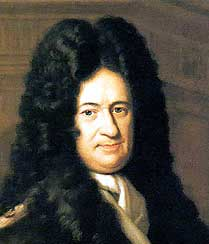
\includegraphics[scale=0.3]{images/Gottfried_Wilhelm_von_Leibniz.jpg}
%\end{minipage}
%&
%\begin{minipage}{0.65\linewidth}
%Né le  1 juillet 1646 à Liepzig, mort le 14 novembre 1716 à Hanovre, Gottfried Liebniz est un esprit universel,
%philosophe, mathématicien, logicien, juriste et diplomate. Il partage avec Isaac Newton la paternité du calcul différentiel et intégral, une controverse sur l'antériorité de la découverte ayant opposé les deux hommes. La notation de Liebniz $\partial f$ est celle qui a été retenue par les mathématiciens, de même que le symbole $\int$ pour l'intégrale.
%\end{minipage}\\
%\multicolumn{2}{l}{\textbf{Isaac Newton}} \\[10pt]
%\begin{minipage}{0.2\linewidth}
%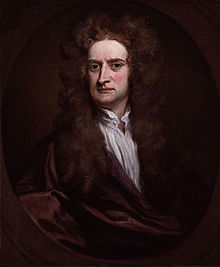
\includegraphics[scale=0.3]{images/isaac_newton.jpg}
%\end{minipage}
%& 
%\begin{minipage}{0.65\linewidth}
%Né le  4 janvier 1643 à Woolsthorpe, mort le 31 mars 1727 à Kensington est un scientifique et philosophe anglais surtout connu pour sa loi de la gravitation universelle. Il a apporté de nombreuses contributions dans le domaine des mathématiques, en particulier la formule du binôme et l'algorithme de recherche des zéros d'une fonction qui porte son nom. Ses travaux sur le calcul infinitésimal on été publiés postérieurement à ceux de Liebniz ce qui a donné lieu à son époque à une dispute sur l'attribution de cette découverte. On lui doit également de nombreux travaux en optique.
%\end{minipage}\\
%
%\multicolumn{2}{l}{\textbf{Stefan Banach}} \\[10pt]
%\begin{minipage}{0.2\linewidth}
%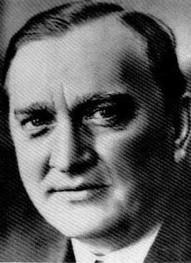
\includegraphics[scale=0.3]{images/banach.jpg}
%\end{minipage}
%& 
%\begin{minipage}{0.65\linewidth}
%Né le 30 mars 1892 à Ostrowsko, mort le 31 août 1945 à Lviv. Banach est un mathématicien fécond, fondateur de l'analyse fonctionnelle. Ses travaux sur les espaces vectoriels topologiques le conduisent à définir les espaces qui portent maintenant son nom. On lui doit également le théorème du point fixe pour les applications contractantes, ainsi que le célèbre paradoxe de Banach-Tarski.
%\end{minipage}
%
%
%\\
%\multicolumn{2}{l}{\textbf{Paul Painlevé}} \\[10pt]
%\begin{minipage}{0.2\linewidth}
%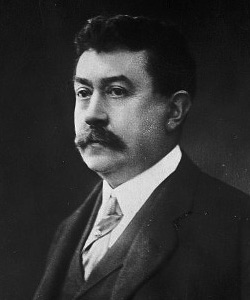
\includegraphics[scale=0.3]{images/painleve.jpg}
%\end{minipage}
%& 
%\begin{minipage}{0.65\linewidth}
%Né le 5 décembre 1863 Paris, mort le 29 octobre 1933 à Paris. Mathématicien et homme politique français né à Paris, Paul Painlevé est aussi un théoricien de l'aviation dont il soutint le développement par son action politique \cite{borel1911aviation}. Les contributions essentielles de Painlevé concernent les équations différentielles ; il résout notamment des équations qui avaient résisté à Poincaré et Picard en introduisant de nouvelles fonctions qui portent désormais le nom de fonctions de Painlevé. Painlevé est également un passionné d'aéronautique : il effectue son baptême de l'air en 1908 comme passager de Wilbur Wright alors que ce dernier bat le record de durée de vol. La carrière politique de Painlevé commence avec l'affaire Dreyfus, dont il est un des plus farouches défenseurs. Il entre au gouvernement en 1915 comme ministre de l'Instruction Publique. Ministre de la guerre en mars 1917, puis Président du conseil en septembre de la même année. Après la fin de la guerre, il anime le cartel des gauches, et préside un temps la chambre des députés. Candidat malheureux à l'élection à la Présidence de la République face à Gaston Doumergue en 1924, il est à nouveau Président du Conseil de 17 avril au 22 novembre 1925. Il est ensuite ministre de la guerre et le premier ministre de l'air. À l'occasion de son décès en octobre 1933, des funérailles nationales sont organisées, et Painlevé est inhumé au Panthéon.
%\end{minipage}
%
%
%
%\end{tabular}


\begin{minipage}{0.2\linewidth}
\begin{center}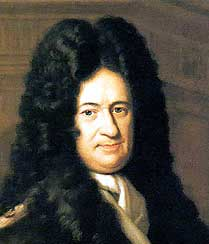
\includegraphics[width=2cm]{images/Gottfried_Wilhelm_von_Leibniz.jpg}\end{center}
\end{minipage}
\begin{minipage}{0.8 \linewidth}
\small{\paragraph*{Gottfried Wilhelm von Leibniz :} Né le 1 juillet 1646 à Liepzig (Electorat de Saxe, Saint-Empire romain germanique), mort le 14 novembre 1716 à Hanovre, Gottfried Liebniz est un esprit universel, philosophe, mathématicien, logicien, juriste et diplomate. Il partage avec Isaac Newton la paternité du calcul différentiel et intégral, une controverse sur l'antériorité de la découverte ayant opposé les deux hommes. La notation de Liebniz $\partial f$ est celle qui a été retenue par les mathématiciens, de même que le symbole $\int$ pour l'intégrale.}
\end{minipage}

\vfill
\begin{minipage}{0.2\linewidth}
\begin{center}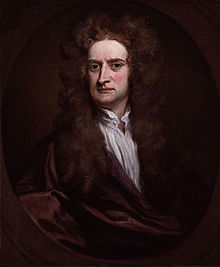
\includegraphics[width=2cm]{images/isaac_newton.jpg}\end{center}
\end{minipage}
\begin{minipage}{0.8\linewidth}
\small{\paragraph*{Isaac Newton :} Né le  4 janvier 1643 à Woolsthorpe (Comté de Lincolnshire, Angleterre), mort le 31 mars 1727 à Kensington (Londres, Angleterre) est un scientifique et philosophe anglais surtout connu pour sa loi de la gravitation universelle. Il a apporté de nombreuses contributions dans le domaine des mathématiques, en particulier la formule du binôme et l'algorithme de recherche des zéros d'une fonction qui porte son nom. Ses travaux sur le calcul infinitésimal on été publiés postérieurement à ceux de Liebniz ce qui a donné lieu à son époque à une dispute sur l'attribution de cette découverte. On lui doit également de nombreux travaux en optique.}
\end{minipage}

\vfill
\begin{minipage}{0.2\linewidth}
\begin{center}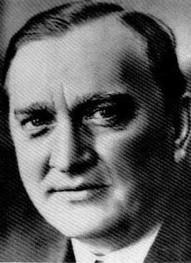
\includegraphics[width=2cm]{images/banach.jpg}\end{center}
\end{minipage}
\begin{minipage}{0.8\linewidth}
\small{\paragraph*{Stefan Banach :} Né le 30 mars 1892 à Ostrowsko (Pologne), mort le 31 août 1945 à Lviv (U.R.S.S.). Banach est un mathématicien fécond, fondateur de l'analyse fonctionnelle. Ses travaux sur les espaces vectoriels topologiques le conduisent à définir les espaces qui portent maintenant son nom. On lui doit également le théorème du point fixe pour les applications contractantes, ainsi que le célèbre paradoxe de Banach-Tarski.}
\end{minipage}
\vfill


\begin{minipage}{0.2\linewidth}
\begin{center}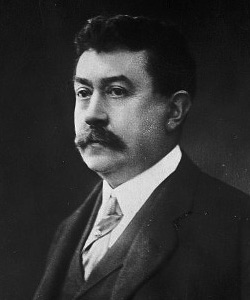
\includegraphics[width=2cm]{images/painleve.jpg}\end{center}
\end{minipage}
\begin{minipage}{0.8\linewidth}
\small{\paragraph*{Paul Painlevé :}Né le 5 décembre 1863 à Paris, mort le 29 octobre 1933 à Paris. Mathématicien et homme politique français né à Paris, Paul Painlevé est aussi un théoricien de l'aviation dont il soutint le développement par son action politique \cite{borel1911aviation}. Les contributions essentielles de Painlevé concernent les équations différentielles ; il résout notamment des équations qui avaient résisté à Poincaré et Picard en introduisant de nouvelles fonctions qui portent désormais le nom de fonctions de Painlevé. Painlevé est également un passionné d'aéronautique : il effectue son baptême de l'air en 1908 comme passager de Wilbur Wright alors que ce dernier bat le record de durée de vol. La carrière politique de Painlevé commence avec l'affaire Dreyfus, dont il est un des plus farouches défenseurs. Il entre au gouvernement en 1915 comme ministre de l'Instruction Publique. Ministre de la guerre en mars 1917, puis Président du conseil en septembre de la même année. Après la fin de la guerre, il est à nouveau Président du Conseil de 17 avril au 22 novembre 1925. Il est ensuite ministre de la guerre et le premier ministre de l'air. À l'occasion de son décès en octobre 1933, des funérailles nationales sont organisées, et Painlevé est inhumé au Panthéon.}
\end{minipage}
\vfill